\documentclass[12pt,a4paper]{article}
 
\usepackage{float}
%für feststellen der figures und tables [H] dranschreiben
\usepackage{units}
%wird so benutzt: 
%\unit[value/Zahl]{dimension/Einheit} oder 
%\unitfrac[value/Zahl]{dimension/Einheit num/Zähler}{dimension/Einheit denum/Nenner} oder
%\nicefrac[fontcommand/Schriftart]{dimension/Einheit num/Zähler}{dimension/Einheit denum/Nenner}

\usepackage{caption}
\usepackage{subcaption}

\usepackage{listings}
 \usepackage{color}

\usepackage[left=2cm,right=2cm,top=2cm,bottom=2cm]{geometry}
\usepackage[utf8]{inputenc}
\usepackage[T1]{fontenc}
\usepackage{lmodern}
\usepackage[ngerman]{babel}
\usepackage{amsmath}
\usepackage{graphicx}
 
%niemals zwei überschriften direkt übereinander schreiben, also immer mindestens in einem satz was sinnvolles unter jede überschrift schreiben (bei den versuchen z.B. das versuchsziel) 
\begin{document}
%deckblatt erstellen.


\begin{titlepage}

\begin{center}
% Oberer Teil der Titelseite:
\includegraphics[width=0.75\textwidth]{logo.pdf}\\[1cm]    	%Logo 

\textsc{\LARGE Bergische Universität Wuppertal}\\[1.5cm]	%Institution

\textsc{\Large Elektronik Praktikum}\\[0.5cm]				%Projekt


\newcommand{\HRule}{\rule{\linewidth}{0.5mm}}
\HRule \\[0.4cm]
{ \huge \bfseries Versuch EP10 Digitalelektronik
Teil 3: Mikrocontroller}\\[0.4cm]				%Titel

\HRule \\[1.5cm]

% Author und Tutor
\begin{minipage}{0.4\textwidth}
\begin{flushleft} \large
\emph{Autoren:}\\
Henrik \textsc{Jürgens} \\
Frederik \textsc{Strothmann}
\end{flushleft}
\end{minipage}
\hfill
\begin{minipage}{0.4\textwidth}
\begin{flushright} \large
\emph{Tutoren:} \\
Hans-Peter \textsc{Kind} \\
Peter \textsc{Knieling} \\
Marius \textsc{Wensing}
\end{flushright}
\end{minipage}

\vfill

% Unterer Teil der Seite/Datum
{\large \today}

\end{center}

\end{titlepage}

\newpage
\tableofcontents
\newpage
\section{Einleitung}
%einleitung zu dem experiment.
%auf die einstellungen, die vor dem versuch gemacht werden, eingehen oder auf eine anleitung dazu verweisen
%es soll immer erwähnt werden um was es in dem Versuch geht und wie das relisiert werden soll
%---------------------------------------------------------------------------------------------
%hinter der einleitung kann der allgemeine theoretische hintergrund in einer zusätzlichen section erklärt werden
%1-----------------------------------------------1
In diesem Versuch geht es um Mikrocontroller und deren Programmierung. Es werden das ansteuern von LEDs, das verwenden von Tastern, die Verwendung eines Oszillators und die Verwendung des ACDs behandelt. Als Versuchsboard wird das Board in Abbildung \ref{fig:board} verwendet.

%In diesem Versuch soll zu jedem Arbeitsschritt eine kurze Beobachtung dokumentiert werden, sowie auch der Quellcode selber, welcher möglichst gut kommentiert werden soll.

\begin{figure}[H] 
  \centering 	
    \includegraphics[ scale = 0.4]{board.png}
  	\caption[Versuchsboard]{Versuchsboard\footnotemark}
  \label{fig:board}
\end{figure}
\footnotetext{Abbildung entnommen von http://www.atlas.uni-wuppertal.de/$\sim$kind/ep10\_14.pdf am 10.01.2015}

\section{Messen der Arbeitsgeschwindigkeit des PIC18F4455}
%kurz das ziel dieses versuchsteiles ansprechen, damit keine zwei überschriften direkt übereinander stehen!
%bei schwierigeren versuchen kann auch der theoretische hintergrund erläutert werden. (mit formeln, herleitungen und erklärungen)

In diesem Versuchsabschnitt wird die Arbeitsgeschwindigkeit des Mikrcontrollers untersucht, dafür wird eine LED mit verschiedenen Schleifen und einem delay-Befehlen an und aus geschaltet.

\subsection{Schnellstmögliches Programm, ohne Verzögerungsbefehle}
%kurz das ziel dieses versuchsteiles ansprechen, damit keine zwei überschriften direkt übereinander stehen!
%bei schwierigeren versuchen kann auch der theoretische hintergrund erläutert werden. (mit formeln, herleitungen und erklärungen)

In diesem Versuchsteil wird einer LED abwechselnd der Zustand 'AN' und 'AUS' zugewiesen. Dies geschieht mit einer 'while(1)' Schleife.

\subsubsection*{Verwendete Geräte}
%(immer) eine skizze oder ein foto einfügen, die geräte/materialien !nummerieren! und z.b. eine legende dazu schreiben, besser wäre es das ganze in einem Fließtext gut zu beschreiben.
%falls am anfang des versuches nicht klar ist, was alles verwendet wird, wenn möglich erst am ende ein großes foto von den verwendeten materialien machen!\\

Es werden ein Netzgerät, ein PC, ein Verbindungskabel, ein Oszillsokop und das Versuchsboard verwendet.

\subsubsection*{Versuchsaufbau}
%skizze zum versuchsaufbau (oder foto) einfügen,   es muss erklärt werden wie das ganze funktioniert und welche speziellen einstellungen verwendet wurden (z.b. welche knöpfe an den geräten für die messung verdreht wurden)

In allen Versuchsteilen wird das Board in Abbilung \ref{fig:board_2} verwendet. Der Versuchsaufbau ändert sich bis auf die Verkabelung nicht.

\begin{figure}[H] 
  \centering 	
    \includegraphics[ scale = 0.4]{board.png}
  	\caption[Versuchsboard]{Versuchsboard\footnotemark}
  \label{fig:board_2}
\end{figure}
\footnotetext{Abbildung entnommen von http://www.atlas.uni-wuppertal.de/$\sim$kind/ep10\_14.pdf am 10.01.2015}

\subsubsection*{Quellcode}

Der Quellcode zum einfachen testen der Geschwindigkeit des Boards.

\lstset{language=C, basicstyle=\tiny}
\begin{lstlisting}[caption = {Einfacher Geschwindigkeitstest} \label{lst:g_1},captionpos=b]
    // Implementierung der eigenen Funktion
    void test_speed_1(){
    	TRISB = 0b00000000;
    	
    	while(1){
    		LATB = 0b1111111;		// In dieser Schleife sollen die LEDs moeglichst
    		LATB = 0b0000000;		// schnell an und aus geschaltet werden.
    	}//end of while(1)
    }//end of function test_speed_1()
\end{lstlisting}

\subsubsection*{Versuchsdurchführung}
%erklären, !was! wir machen, !warum! wir das machen und mit welchem ziel
%(wichtig) präzize erklären, wie bei dem versuch vorgegangen und was gemacht wurde

Der Code \ref{lst:g_1} wird auf den Mikrokontroller geladen. Danach wird Port B über ein Flachbandkabel mit dem LED Port verbunden. Das Board wird an ein Oszilloskop angeschlossen und die Ausgangsfrequenz an den Pins gemessen.


\subsubsection*{Auswertung}
%zuerst !alle! errechneten werte entweder in ganzen sätzen aufzählen, oder in tabellen (übersichtlicher) dargestellen, sowie auf die verwendeten formeln verweisen (die referenzierung der formel kann in der überschrift stehen)
%kurz erwähnen (vor der tabelle), warum wir das ganze ausrechnen bzw. was wir dort ausrechnen
%danach histogramme und plots erstellen, wobei wenn möglich funktionen durch die plots gelegt werden (zur not können auch splines benutzt werden, was aber angegeben werden muss)
%bei fits immer die funktion und das reduzierte chiquadrat mit angegeben, wobei auf verständlichkeit beim entziffern der zehnerpotenzen geachtet werden muss z.b. f(x)=(wert+-fehler)\cdot10^{irgendeine zahl}\cdot x + (wert+-fehler)\cdot10^{irgendeine zahl}
%bei jedem fit erklären, nach welchem zusammenhang gefittet wurde und warum!
%bei plots darauf achten, dass die achsenbeschriftung (auch die tics) die richtige größe haben und die legende im plot nicht die messwerte verdeckt
%kurz die aufgabenstellung abhandeln
%2-----------------------------------------------2

Die LEDs leuchteten, es war kein Flackern zu erkennen. Die Messung der Frquenz mit dem Oszilloskop ergab \unit[2,4]{GHz}. Der Verlauf des Signals ist in Abbildung \ref{fig:g_1} zu sehen.

\begin{figure}[H] 
  \centering 	
    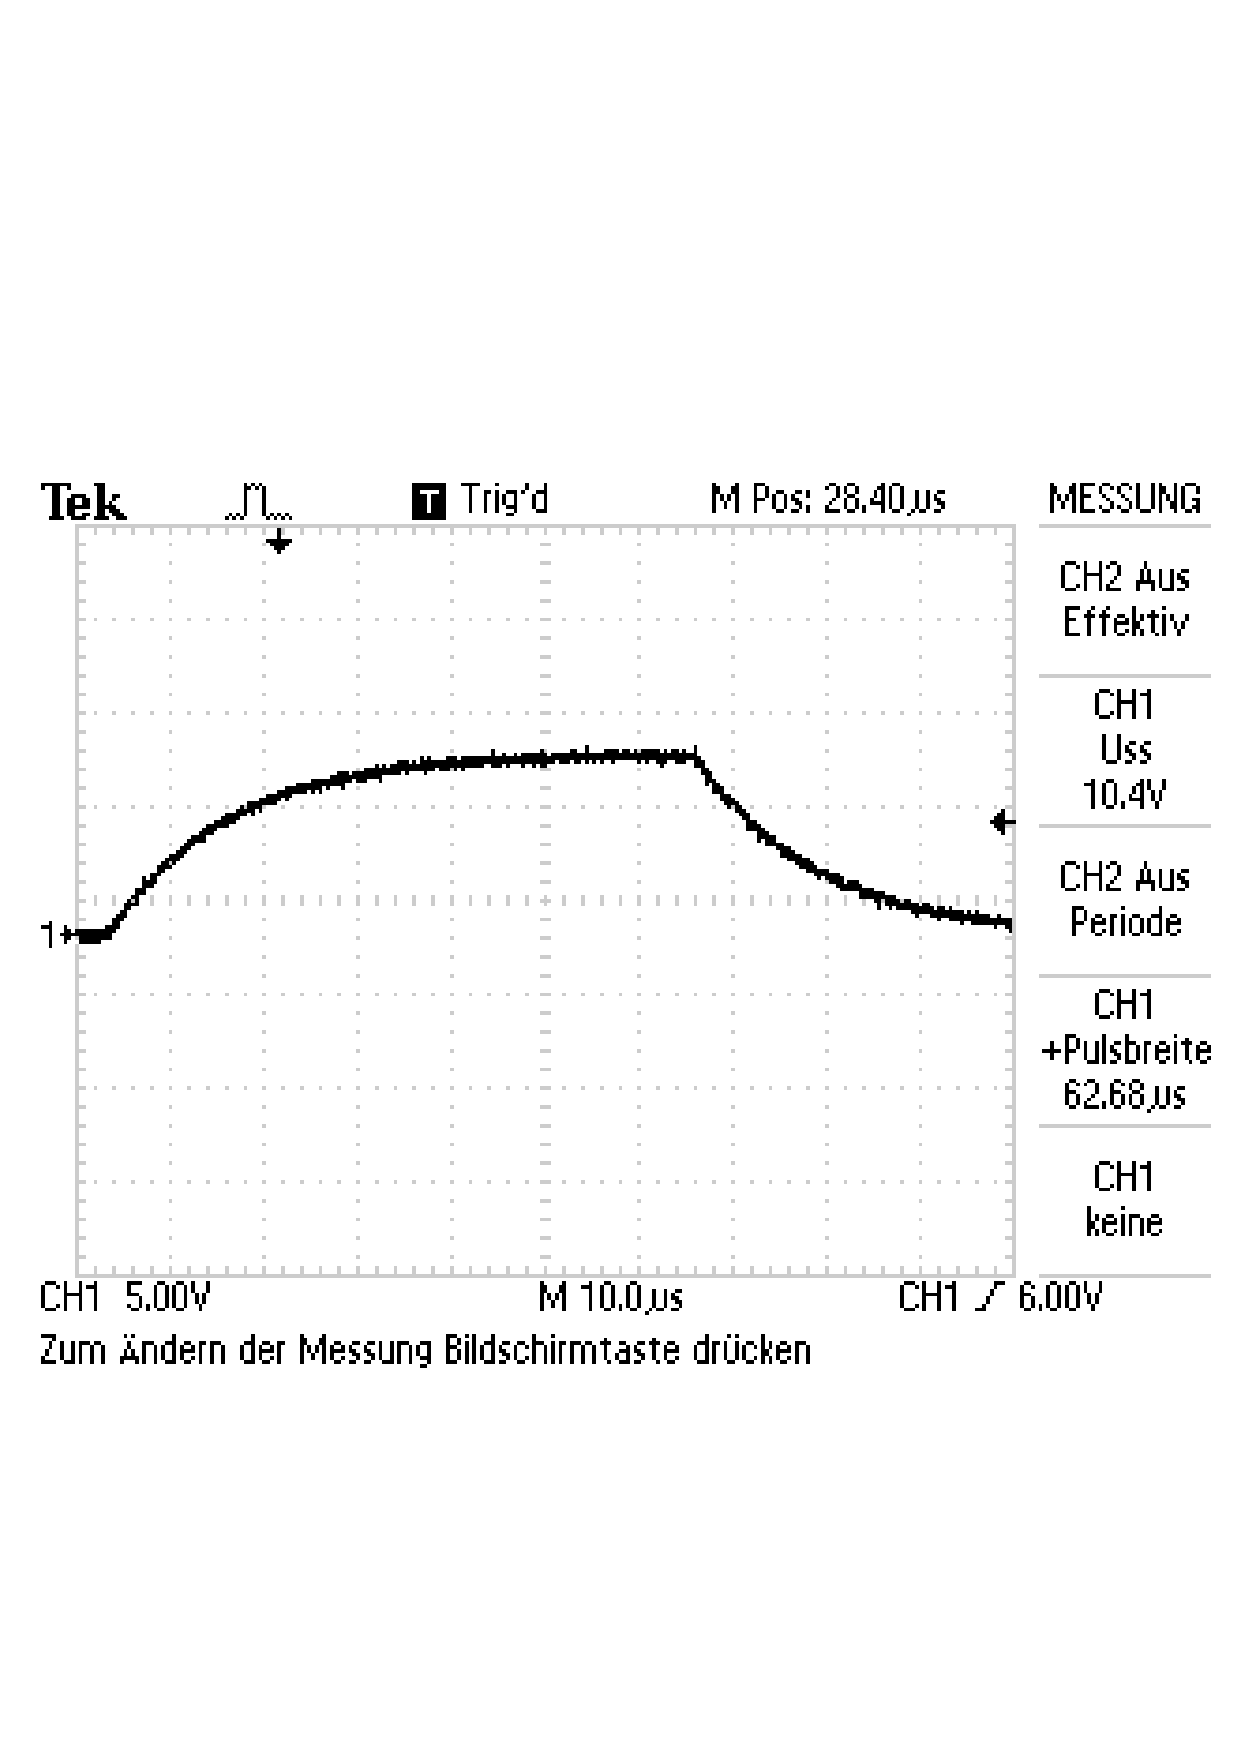
\includegraphics[trim = 0mm 50mm 0mm 50mm, clip, scale = 0.4]{TEK0000.pdf}
  	\caption[Aufnahme des Signals]{Aufnahme des Signals} 
  \label{fig:g_1}
\end{figure}



\subsection{Programm mit Verzögerungsbefehlen aus for-Schleifen}
%kurz das ziel dieses versuchsteiles ansprechen, damit keine zwei überschriften direkt übereinander stehen!
%bei schwierigeren versuchen kann auch der theoretische hintergrund erläutert werden. (mit formeln, herleitungen und erklärungen)

In diesem Versuchsteil soll eine LED  mit Verzögerung ein- und ausgeschaltet werden. Die Pausen werden mit Hilfe einer for-Schleife realisiert. Um die Länge der Verzögerung einzustellen wird der Befehl Nop() verwendet. Dieser sorgt dafür, dass der Mikocontroller für einen Taktzyklus aussetzt.

\subsubsection*{Verwendete Geräte}
%(immer) eine skizze oder ein foto einfügen, die geräte/materialien !nummerieren! und z.b. eine legende dazu schreiben, besser wäre es das ganze in einem Fließtext gut zu beschreiben.
%falls am anfang des versuches nicht klar ist, was alles verwendet wird, wenn möglich erst am ende ein großes foto von den verwendeten materialien machen!\\

Es werden ein Netzgerät, ein PC, ein Verbindungskabel, ein Oszillsokop und das Versuchsboard verwendet.


\subsubsection*{Quellcode}

Quellcode zum testen der Geschwindigkeit des Boards mit einer for-Schleife und dem Nop()-Befehl.

\lstset{language=C, basicstyle=\tiny}
\begin{lstlisting}[caption = {Geschwindigkeitstest mit einer for-Schleife} \label{lst:g_2},captionpos=b]
void test_speed_for(){
	int i;
	TRISB = 0b00000000;
	
	while(1){
		for(i=0; i<10; i++){
			Nop();			// zum Verzoegern von 10 Taktzyklen
		}
	
		LATB = 0b1111111;
		
		for(i=0; i<10; i++){
			Nop();			// zum Verzoegern von 10 Taktzyklen
		}
		
		LATB = 0b0000000;
	}//end of while(1)
}//end of function test_speed_for()
\end{lstlisting}


\subsubsection*{Versuchsdurchführung}
%erklären, !was! wir machen, !warum! wir das machen und mit welchem ziel
%(wichtig) präzize erklären, wie bei dem versuch vorgegangen und was gemacht wurde

Der Code \ref{lst:g_2} wird auf den Mikrokontroller geladen. Port B wird mit dem LED Port über ein Flachbandkabel verbunden. Dann wird das Board an ein Oszilloskop angeschlossen und die Ausgangsfrequenz an den Pins gemessen.

\subsubsection*{Auswertung}
%zuerst !alle! errechneten werte entweder in ganzen sätzen aufzählen, oder in tabellen (übersichtlicher) dargestellen, sowie auf die verwendeten formeln verweisen (die referenzierung der formel kann in der überschrift stehen)
%kurz erwähnen (vor der tabelle), warum wir das ganze ausrechnen bzw. was wir dort ausrechnen
%danach histogramme und plots erstellen, wobei wenn möglich funktionen durch die plots gelegt werden (zur not können auch splines benutzt werden, was aber angegeben werden muss)
%bei fits immer die funktion und das reduzierte chiquadrat mit angegeben, wobei auf verständlichkeit beim entziffern der zehnerpotenzen geachtet werden muss z.b. f(x)=(wert+-fehler)\cdot10^{irgendeine zahl}\cdot x + (wert+-fehler)\cdot10^{irgendeine zahl}
%bei jedem fit erklären, nach welchem zusammenhang gefittet wurde und warum!
%bei plots darauf achten, dass die achsenbeschriftung (auch die tics) die richtige größe haben und die legende im plot nicht die messwerte verdeckt
%kurz die aufgabenstellung abhandeln
%2-----------------------------------------------2

Die LEDs leuchteten, es war kein Flackern zu erkennen. Die Messung der Frequenz mit dem Oszilloskop ergab \unit[28,9]{kHz}. Der Verlauf des Signals ist in Abbildung \ref{fig:g_2} zu sehen.

\begin{figure}[H] 
  \centering 	
    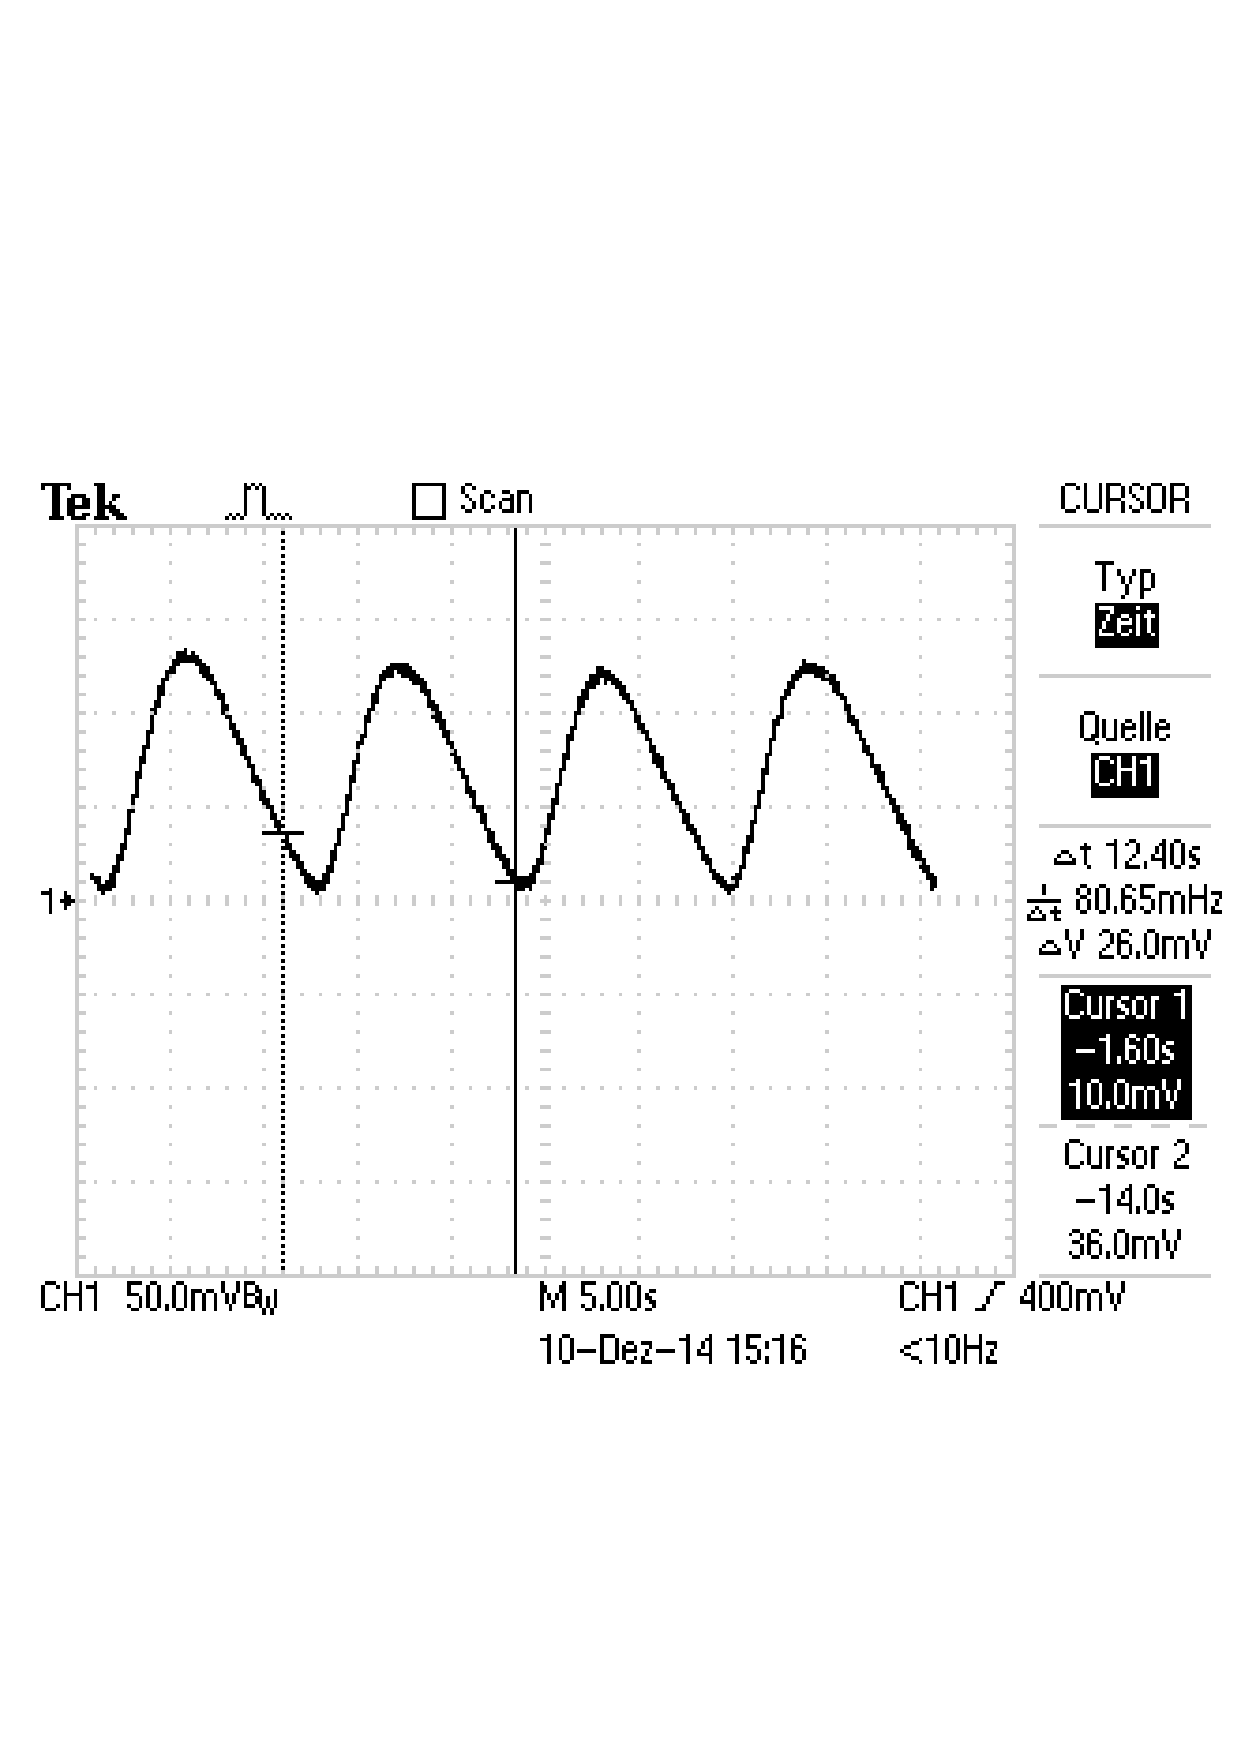
\includegraphics[trim = 0mm 50mm 0mm 50mm, clip, scale = 0.4]{TEK0001.pdf}
  	\caption[Aufnahme des Signals]{Aufnahme des Signals} 
  \label{fig:g_2}
\end{figure}

\subsection{Programm mit Compiler-Verzögerungsbefehlen}

In diesem Versuchsteil soll eine Verzögerung des Ein- und Ausschaltvorgangs der LED mit dem Compiler-Verzögerungsbefehlen realisiert werden. Bei dieser Art der Verzögerung wird eine bestimmte Anzahl von Taktzyklen ausgesetzt. Zur Erzeugung der Verzögerung werden die folgenden Befehle (unit kann Werte von 0 bis 255 annehmen) verwendet.

\begin{itemize}
\item	Delay1TCY() oder Nop() delay von einem instruction cycle

\item	Delay10TCYx(unit) delay von unit $\times$ 10 instruction cycle

\item	Delay100TCYx(unit) delay von unit $\times$ 100 instruction cycle

\item	Delay10KTCYx(unit) delay von unit $\times$ 1000 instruction cycle

\item	Delay10KTCYx(unit) delay von unit $\times$ 10000 instruction cycle

\end{itemize}

\subsubsection*{Verwendete Geräte}

Es werden ein Netzgerät, ein PC, ein Verbindungskabel, ein Oszillsokop und das Versuchsboard verwendet.

\subsubsection*{Quellcode}

Quellcode zum testen der Compiler-Verzögerungsbefehle.

\lstset{language=C, basicstyle=\tiny}
\begin{lstlisting}[caption = {Geschwindigkeitstest mit Compiler-Verzögerungsbefehlen} \label{lst:g_3},captionpos=b]
void test_speed_delay_1(){
	int i;
	TRISB = 0b00000000;
	
	while(1){
		Delay10TCYx(100);
		LATBbits.LATB0 = 1;
		Delay100TCYx(100);
		LATBbits.LATB1 = 1;
		Delay1KTCYx(100);
		LATBbits.LATB2 = 1;
		Delay10KTCYx(100);
		LATBbits.LATB3 = 1;
		Delay10TCYx(255);
		LATBbits.LATB4 = 1;
		Delay100TCYx(255);
		LATBbits.LATB5 = 1;
		Delay1KTCYx(255);
		LATBbits.LATB6 = 1;
		Delay10KTCYx(255);
		LATBbits.LATB7 = 1;	// es wurden dierekt mehrere Verzoegerungsbefehle verwendet
		Delay10KTCYx(100);	// wurde im ersten Durchlauf auskommentiert
		
		LATB = 0b00000000;
		
	}//end of while(1)
}//end of function test_speed_delay_1()
\end{lstlisting}


\subsubsection*{Versuchsdurchführung}

Der Code \ref{lst:g_3} wird auf den Mikrokontroller geladen. Port B wird mit Port LED, über ein Flachbandkabel verbunden. Das Board wird an ein Oszilloskop angeschlossen und die Ausgangsfrequenz an den Pins gemessen. Dann wird die in Code \ref{lst:g_3} erwähnte Zeile einkommentiert und die Frequenz mit dem  Oszilloskop gemessen.


\subsubsection*{Auswertung}

Die Spannung wurde bei B6 abgegriffen, im ersten Durchlauf wurde eine Frquenz von 3,04Hz gemessen. Der Verlauf des Signals ist in Abbildung \ref{fig:g_3} zu sehen. Im zweitem Durchlauf wurde eine Frequez von 2,42Hz gemessen. Der Verlauf des Signals ist in Abbildung \ref{fig:g_4} zu sehen.

\begin{figure}[H]
\centering
\begin{subfigure}[b]{0.45\textwidth} 	
  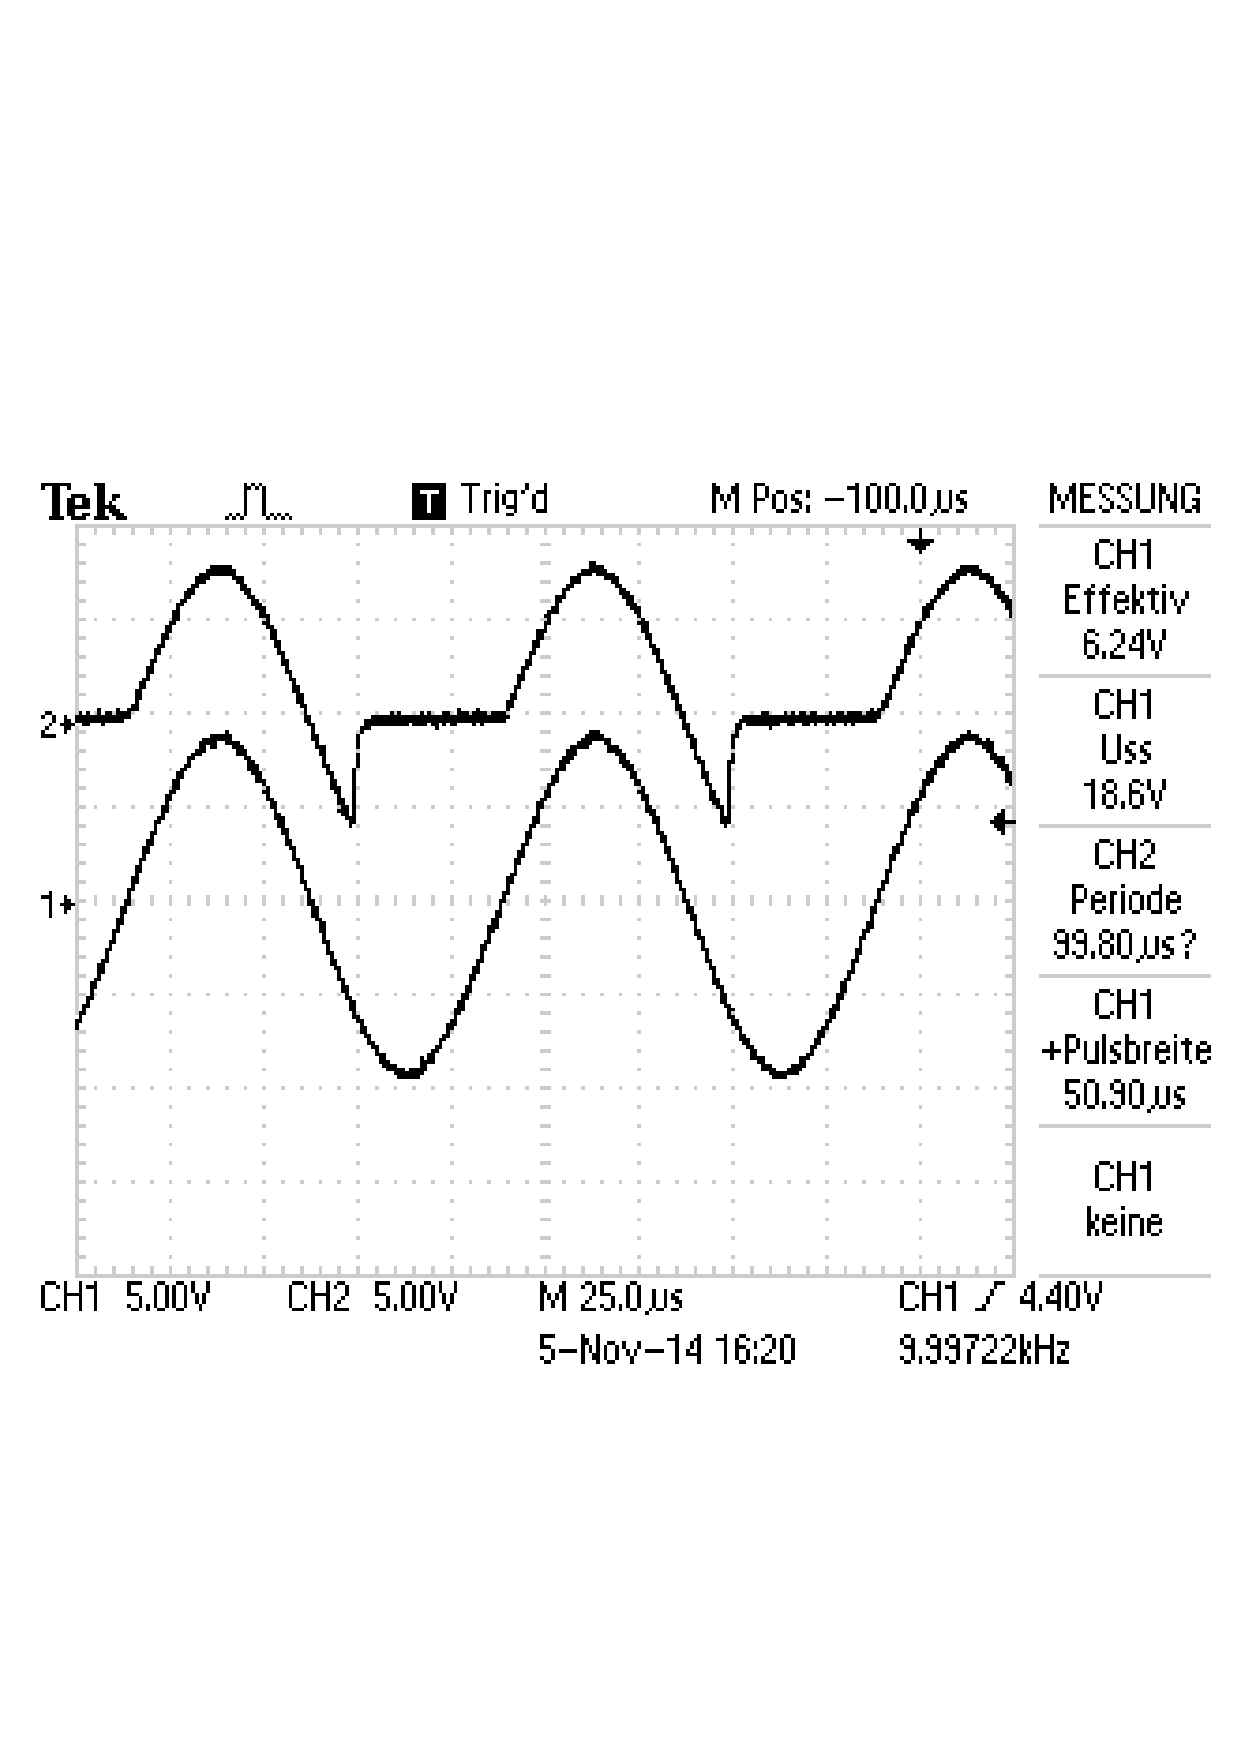
\includegraphics[trim = 0mm 50mm 0mm 50mm, clip, scale = 0.4]{TEK0002.pdf}
  \caption[Aufnahme des Signals, mit Auskommentierung]{Aufnahme des Signals, mit Auskommentierung} 
  \label{fig:g_3}
\end{subfigure}
\hfill
\begin{subfigure}[b]{0.45\textwidth}	
   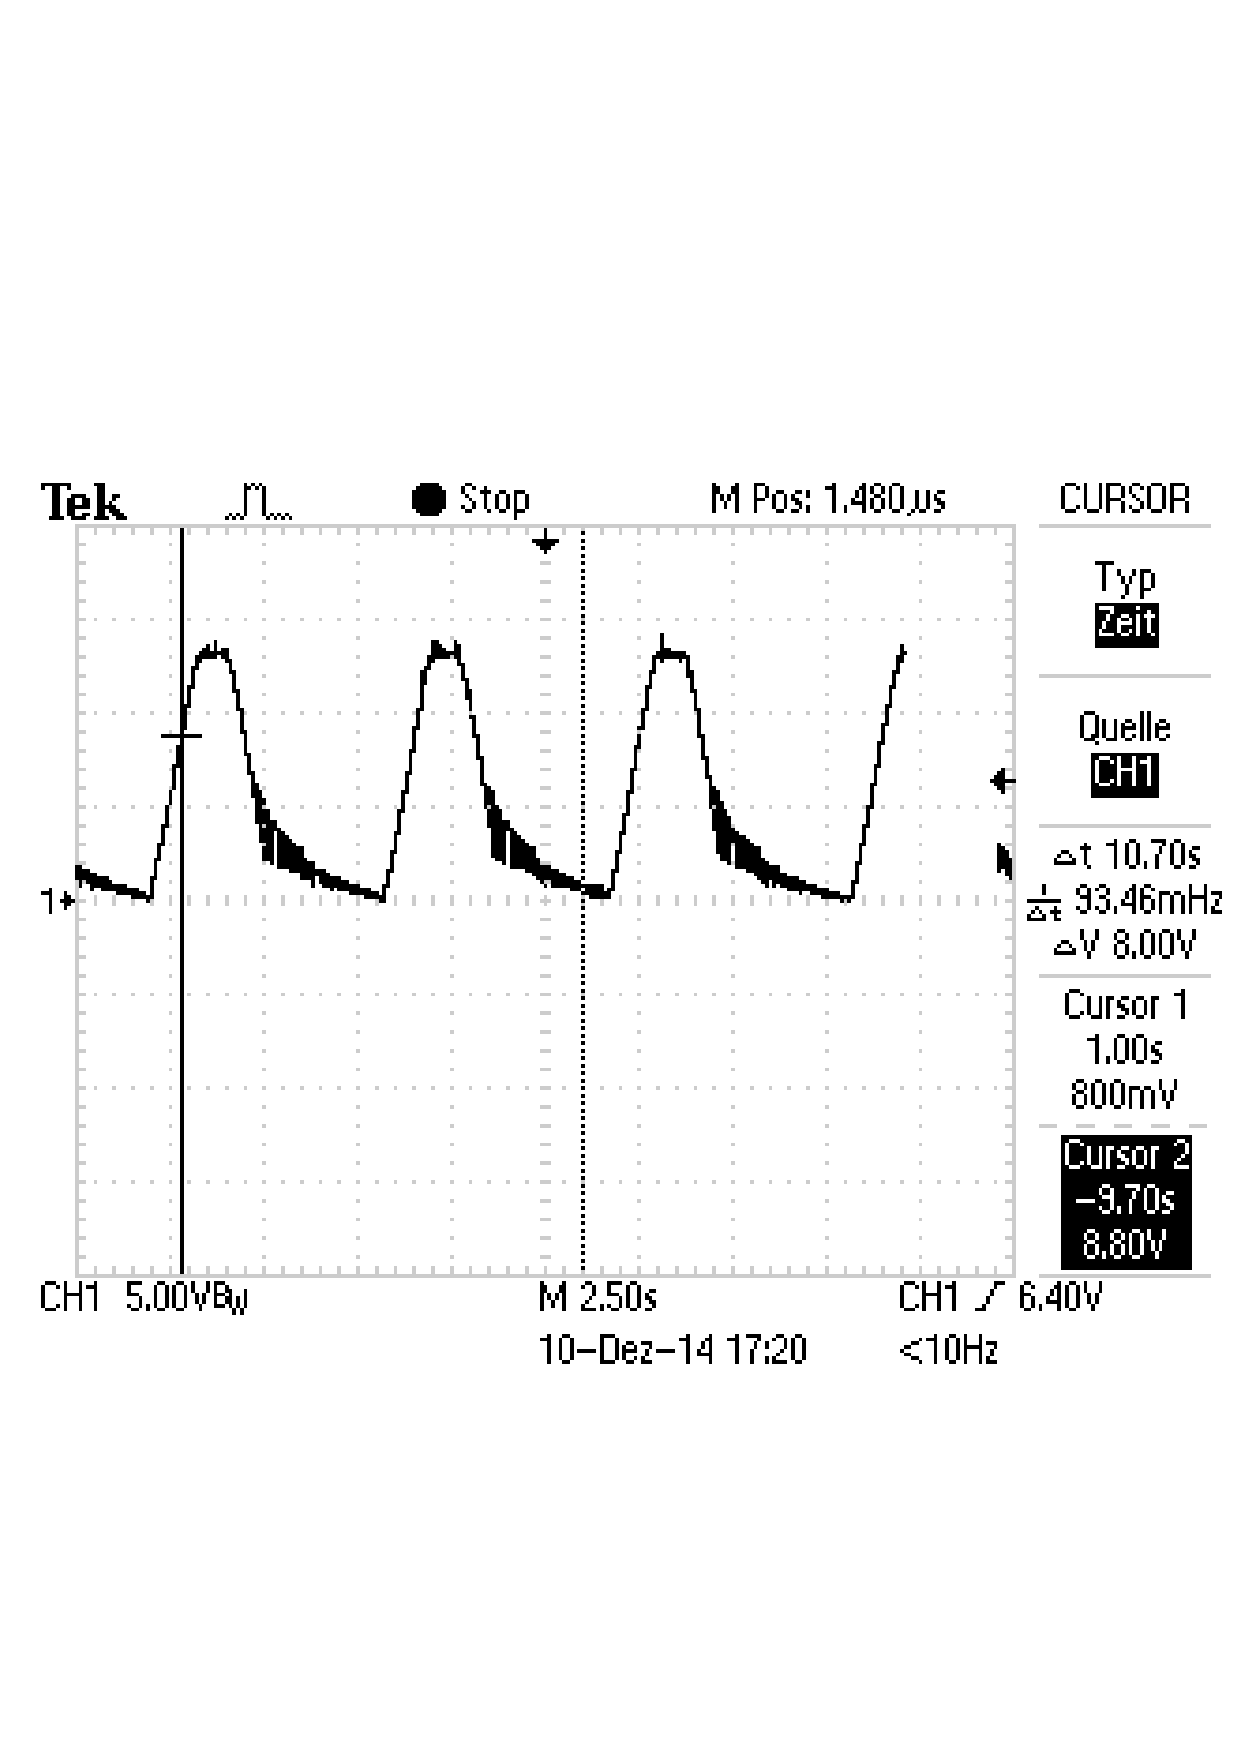
\includegraphics[trim = 0mm 50mm 0mm 50mm, clip, scale = 0.4]{TEK0004.pdf}
  \caption[Aufnahme des Signals, ohne Auskommentierung]{Aufnahme des Signals, ohne Auskommentierung} 
  \label{fig:g_4}
\end{subfigure}
\end{figure}

Bei beiden Versionen leuchteten die ersten drei LEDs und die Restlichen blinkten.

\subsection{Programm mit fertigen Verzögerungsbefehlen}
%kurz das ziel dieses versuchsteiles ansprechen, damit keine zwei überschriften direkt übereinander stehen!
%bei schwierigeren versuchen kann auch der theoretische hintergrund erläutert werden. (mit formeln, herleitungen und erklärungen)

In diesem Versuchsteil soll das An- und Ausschalten der LED mit verschiedenen Verzögerungsbefehlen realisiert werden. Verzögerungsbefehle sorgen für eine Verzögerung von einer bestimmten Zeitspannne und nicht wie Vorher für ein Aussetzen einer Anzahl von Taktzyklen. Es werden die folgenden Befehle (unit kann Werte von 0 bis 255) verwendet.

\begin{itemize}
\item	delay us(unit) verzögert um unit Mikrosekunden

\item	delay 10us(unit) verzögert um unit $\times$ 10 Mikrosekunden

\item	delay ms(unit) verzögert um unit Millisekunden
\end{itemize}

\subsubsection*{Verwendete Geräte}
%(immer) eine skizze oder ein foto einfügen, die geräte/materialien !nummerieren! und z.b. eine legende dazu schreiben, besser wäre es das ganze in einem Fließtext gut zu beschreiben.
%falls am anfang des versuches nicht klar ist, was alles verwendet wird, wenn möglich erst am ende ein großes foto von den verwendeten materialien machen!\\

Es werden ein Netzgerät, ein PC, ein Verbindungskabel, ein Oszillsokop und das Versuchsboard verwendet.


\subsection*{Messergebnisse}
\begin{table}[H]
\centering
\begin{tabular}{|c|c|}
	\hline
	    Befehl     & Pulsbreite/$\mu$s \\ \hline\hline
	 delay\_us(1)  &       1,66        \\ \hline
	 delay\_us(2)  &       2,66        \\ \hline
	delay\_10us(0) &       1,91        \\ \hline
	delay\_10us(1) &       12,4        \\ \hline
	 delay\_ms(0)  &       3,00        \\ \hline
	 delay\_ms(1)  &       995,9       \\ \hline
\end{tabular} 
\caption{Pulsbreiten der Verschiedenen Befehle}
\label{tab:puls_1}
\end{table}


\subsubsection*{Quellcode}

Quellcode zum testen der fertigen Verzögerungsbefehlen.

\lstset{language=C, basicstyle=\tiny}
\begin{lstlisting}[caption = {Geschwindigkeitstest mit den fertigen Verzögerungsbefehlen} \label{lst:g_4},captionpos=b]
void test_speed_delay_3(){
	TRISB = 0b00000000;		// Quellcode war vorgegeben
	
	while(1){
		delay_us(25);
		LATBbits.LATB0 = 1;
		delay_us(25);
		LATBbits.LATB1 = 0;
	}//end of while(1)
}//end of function test_speed_delay_3()
\end{lstlisting}



\subsubsection*{Versuchsdurchführung}
%erklären, !was! wir machen, !warum! wir das machen und mit welchem ziel
%(wichtig) präzize erklären, wie bei dem versuch vorgegangen und was gemacht wurde

Der Code \ref{lst:g_4} wird auf den Mikrokontroller geladen und Port B wird mit dem LED Port verbunden. Dann wird das Board an ein Oszilloskop angeschlossen und die Pulsbreite der Signale an den Pins gemessen. Dieser Prozess wir mit verschiednen Verzögerungsbefehlen wiederholt.


\subsubsection*{Auswertung}
%zuerst !alle! errechneten werte entweder in ganzen sätzen aufzählen, oder in tabellen (übersichtlicher) dargestellen, sowie auf die verwendeten formeln verweisen (die referenzierung der formel kann in der überschrift stehen)
%kurz erwähnen (vor der tabelle), warum wir das ganze ausrechnen bzw. was wir dort ausrechnen
%danach histogramme und plots erstellen, wobei wenn möglich funktionen durch die plots gelegt werden (zur not können auch splines benutzt werden, was aber angegeben werden muss)
%bei fits immer die funktion und das reduzierte chiquadrat mit angegeben, wobei auf verständlichkeit beim entziffern der zehnerpotenzen geachtet werden muss z.b. f(x)=(wert+-fehler)\cdot10^{irgendeine zahl}\cdot x + (wert+-fehler)\cdot10^{irgendeine zahl}
%bei jedem fit erklären, nach welchem zusammenhang gefittet wurde und warum!
%bei plots darauf achten, dass die achsenbeschriftung (auch die tics) die richtige größe haben und die legende im plot nicht die messwerte verdeckt
%kurz die aufgabenstellung abhandeln
%2-----------------------------------------------2

Es wurde Quellcode \ref{lst:g_4} verwendet. Der Befehl \textbf{delay\_us(25)} wurde der Reihe nach durch die Folgenden ersetzt.

\begin{itemize}
\item	delay\_us(1)

\item	delay\_us(2)

\item	delay\_10us(0)

\item	delay\_10us(1)

\item	delay\_ms(0)

\item	delay\_ms(1)
\end{itemize}
 Die Frequenz wurde bei jedem dieser Befehle gemessen.
 Dabei ergaben sich die Werte in Tabelle \ref{tab:puls_1}. Die Aufnahmen der jeweiligen Signale sind in Abbildung \ref{fig:g_main_1} und Abbildung \ref{fig:g_main_2} zu sehen. Bei allen Befehlen ist die benötigte Zeit 0,6 bis 3 $\mu$s länger als gewünscht.(Bei sehr kleinen Zeiten ergeben sich große relative Abweichungen von der gewünschten Verzögerung.) Dies Begründet sich dadurch, dass die Anzahl der Zyklen, die ausgesetzt werden müssen um die gewünschte Verzögerung zu erreichen, intern berechnet wird. Ein Zyklus dauert 83,33 ns. Der letzte Befehl hat eine gerigere Pulsbreite als 1ms. Bei längeren Verzögerungszeiten sind die Abweichungen zu vernachlässigen.


\begin{figure}[H]
\centering
\begin{subfigure}[b]{0.28\textwidth} 	
  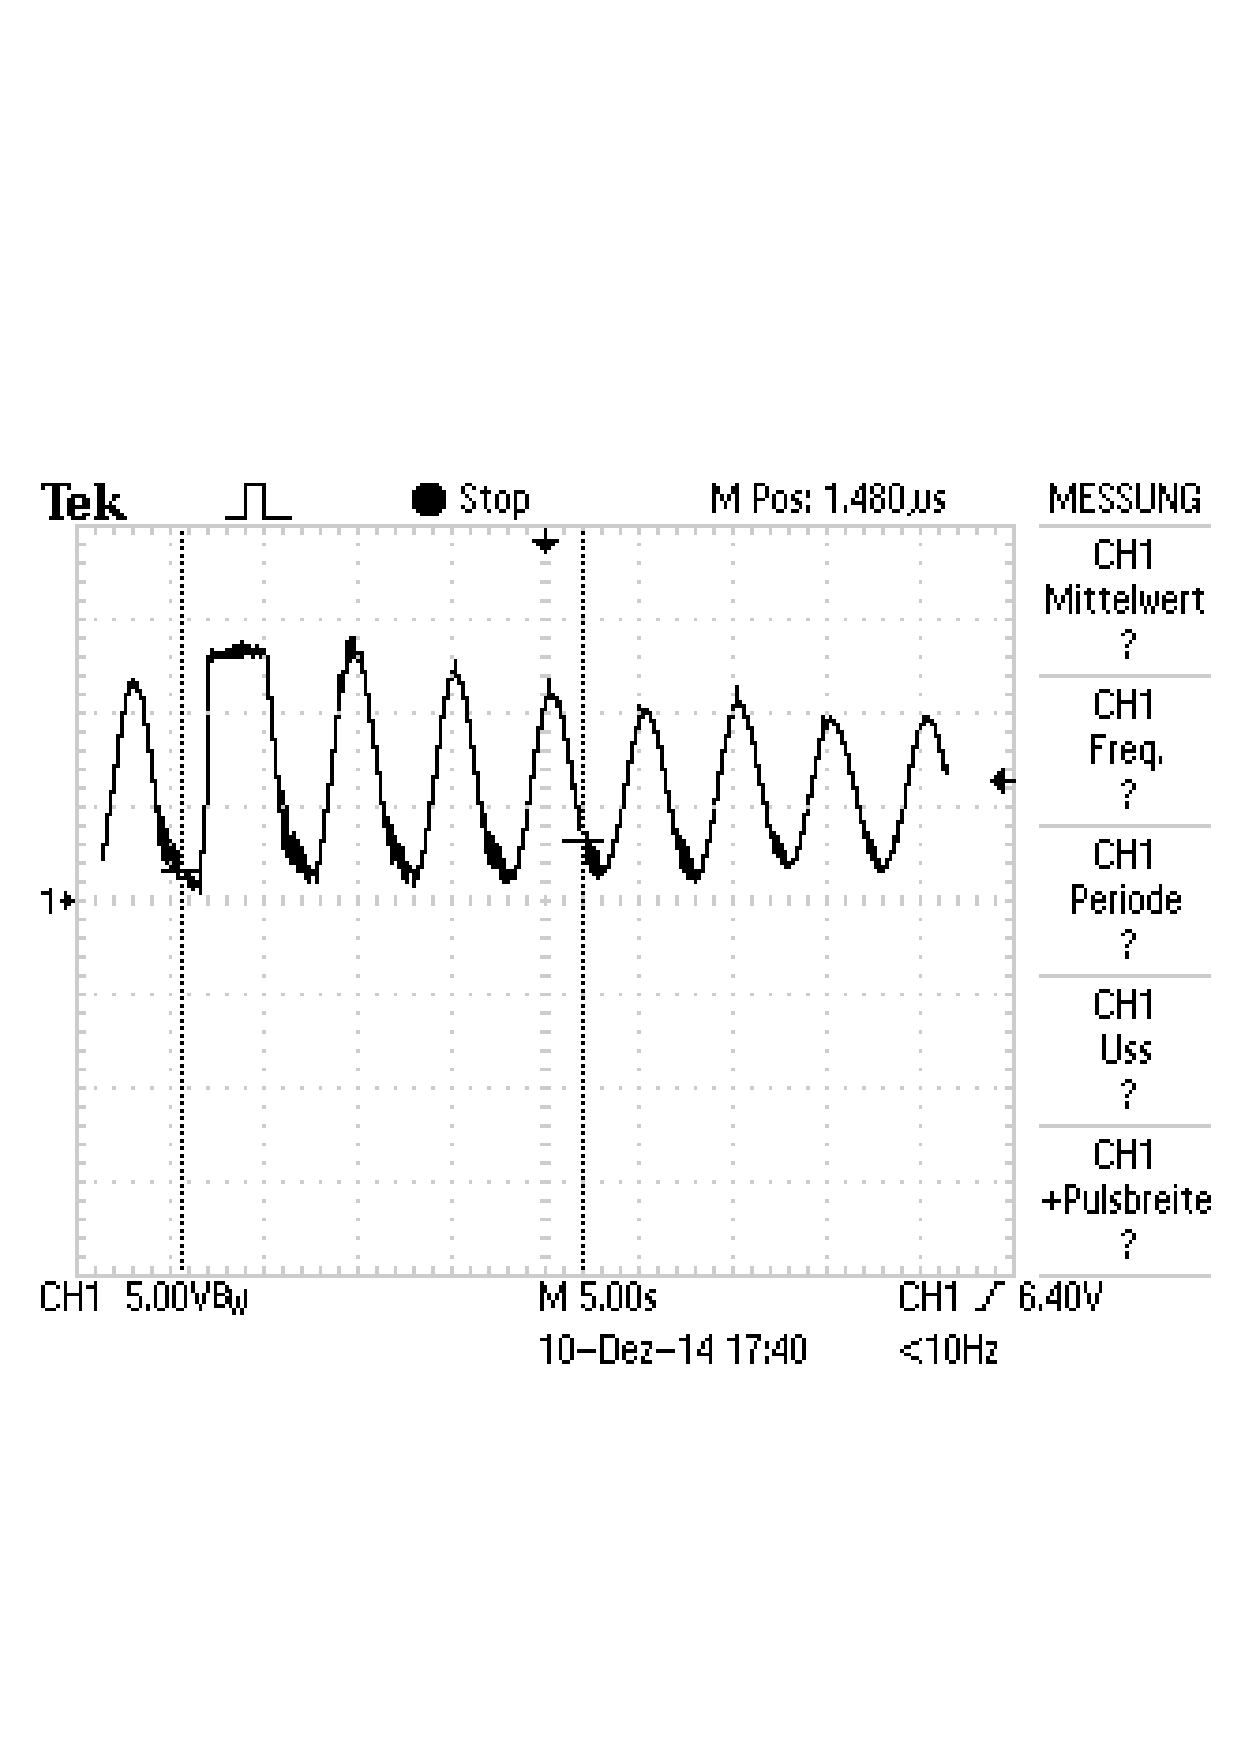
\includegraphics[trim = 0mm 50mm 0mm 50mm, clip, width=\textwidth, scale = 0.4]{TEK0008.pdf}
  \caption[Aufnahme des Signals, für delay\_us(1)]{Aufnahme des Signals, für delay\_us(1)} 
  \label{fig:g_3}
\end{subfigure}
\hfill
\begin{subfigure}[b]{0.28\textwidth}	
   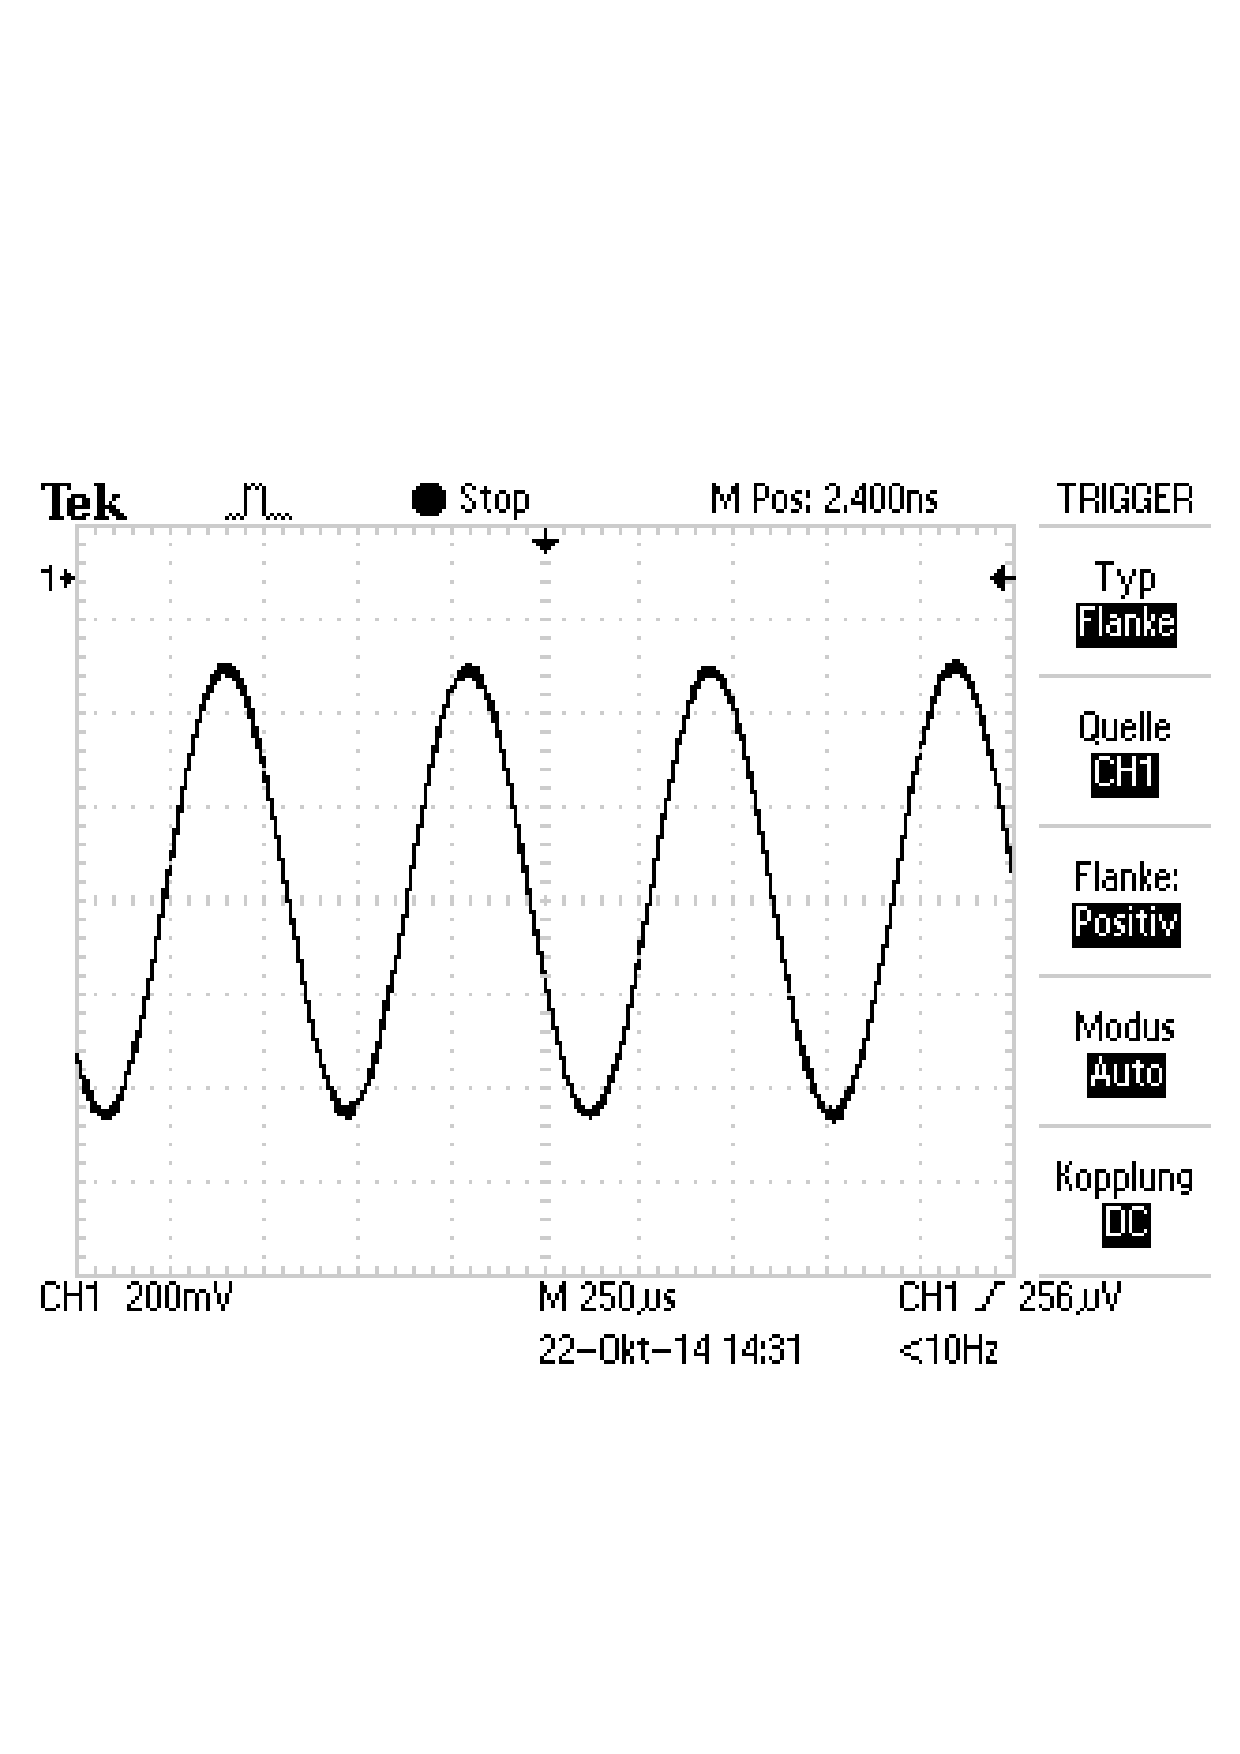
\includegraphics[trim = 0mm 50mm 0mm 50mm, clip, width=\textwidth, scale = 0.4]{TEK0009.pdf}
  \caption[Aufnahme des Signals, für delay\_us(2)]{Aufnahme des Signals, für delay\_us(2)} 
  \label{fig:g_4}
\end{subfigure}
\hfill
\begin{subfigure}[b]{0.28\textwidth} 	
  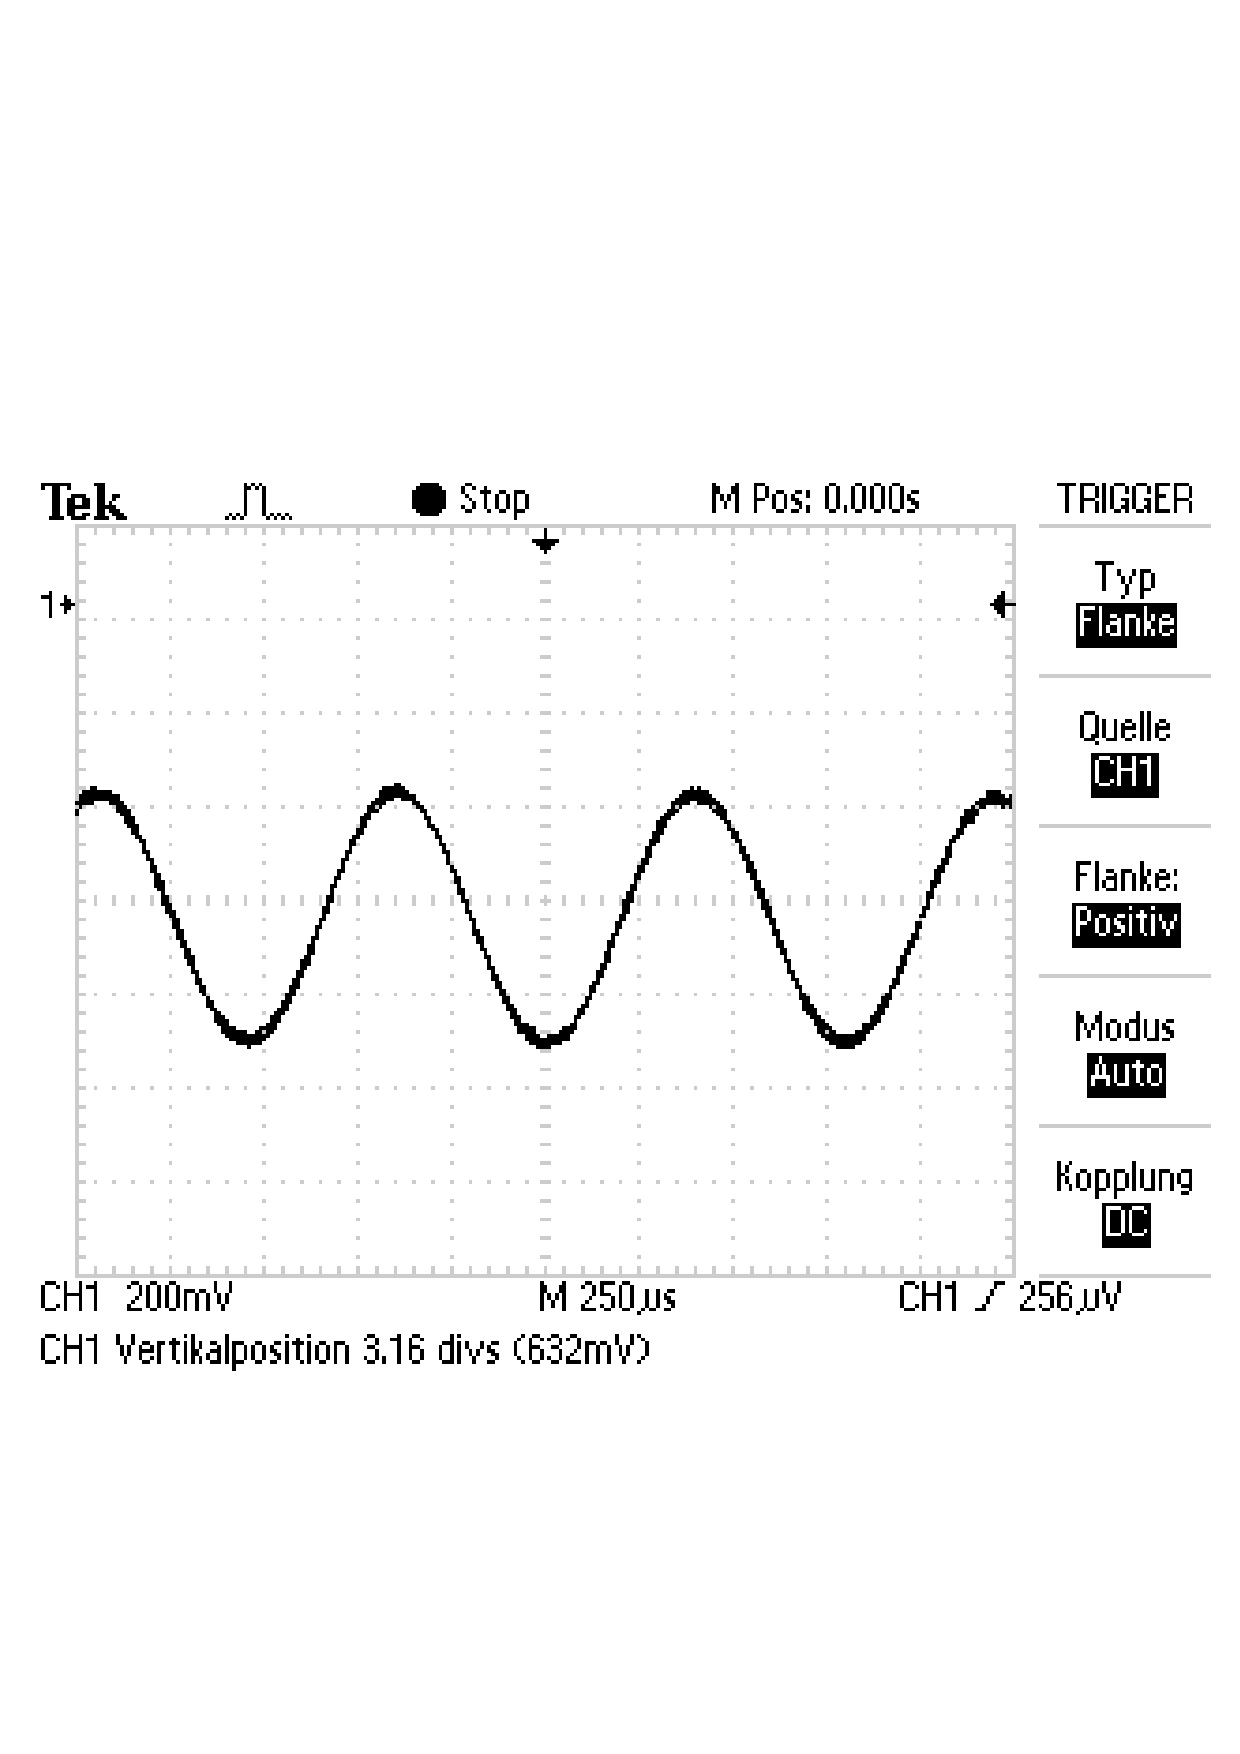
\includegraphics[trim = 0mm 50mm 0mm 50mm, clip, width=\textwidth, scale = 0.4]{TEK0010.pdf}
  \caption[Aufnahme des Signals, für delay\_10us(0)]{Aufnahme des Signals, für delay\_10us(0)} 
  \label{fig:g_3}
\end{subfigure}
\caption{Oszilloskopaufnahmen für delay\_us(1), delay\_us(2) und delay\_10us(0)}
\label{fig:g_main_1}
\end{figure}


\begin{figure}[H]
\centering
\begin{subfigure}[b]{0.28\textwidth} 	
  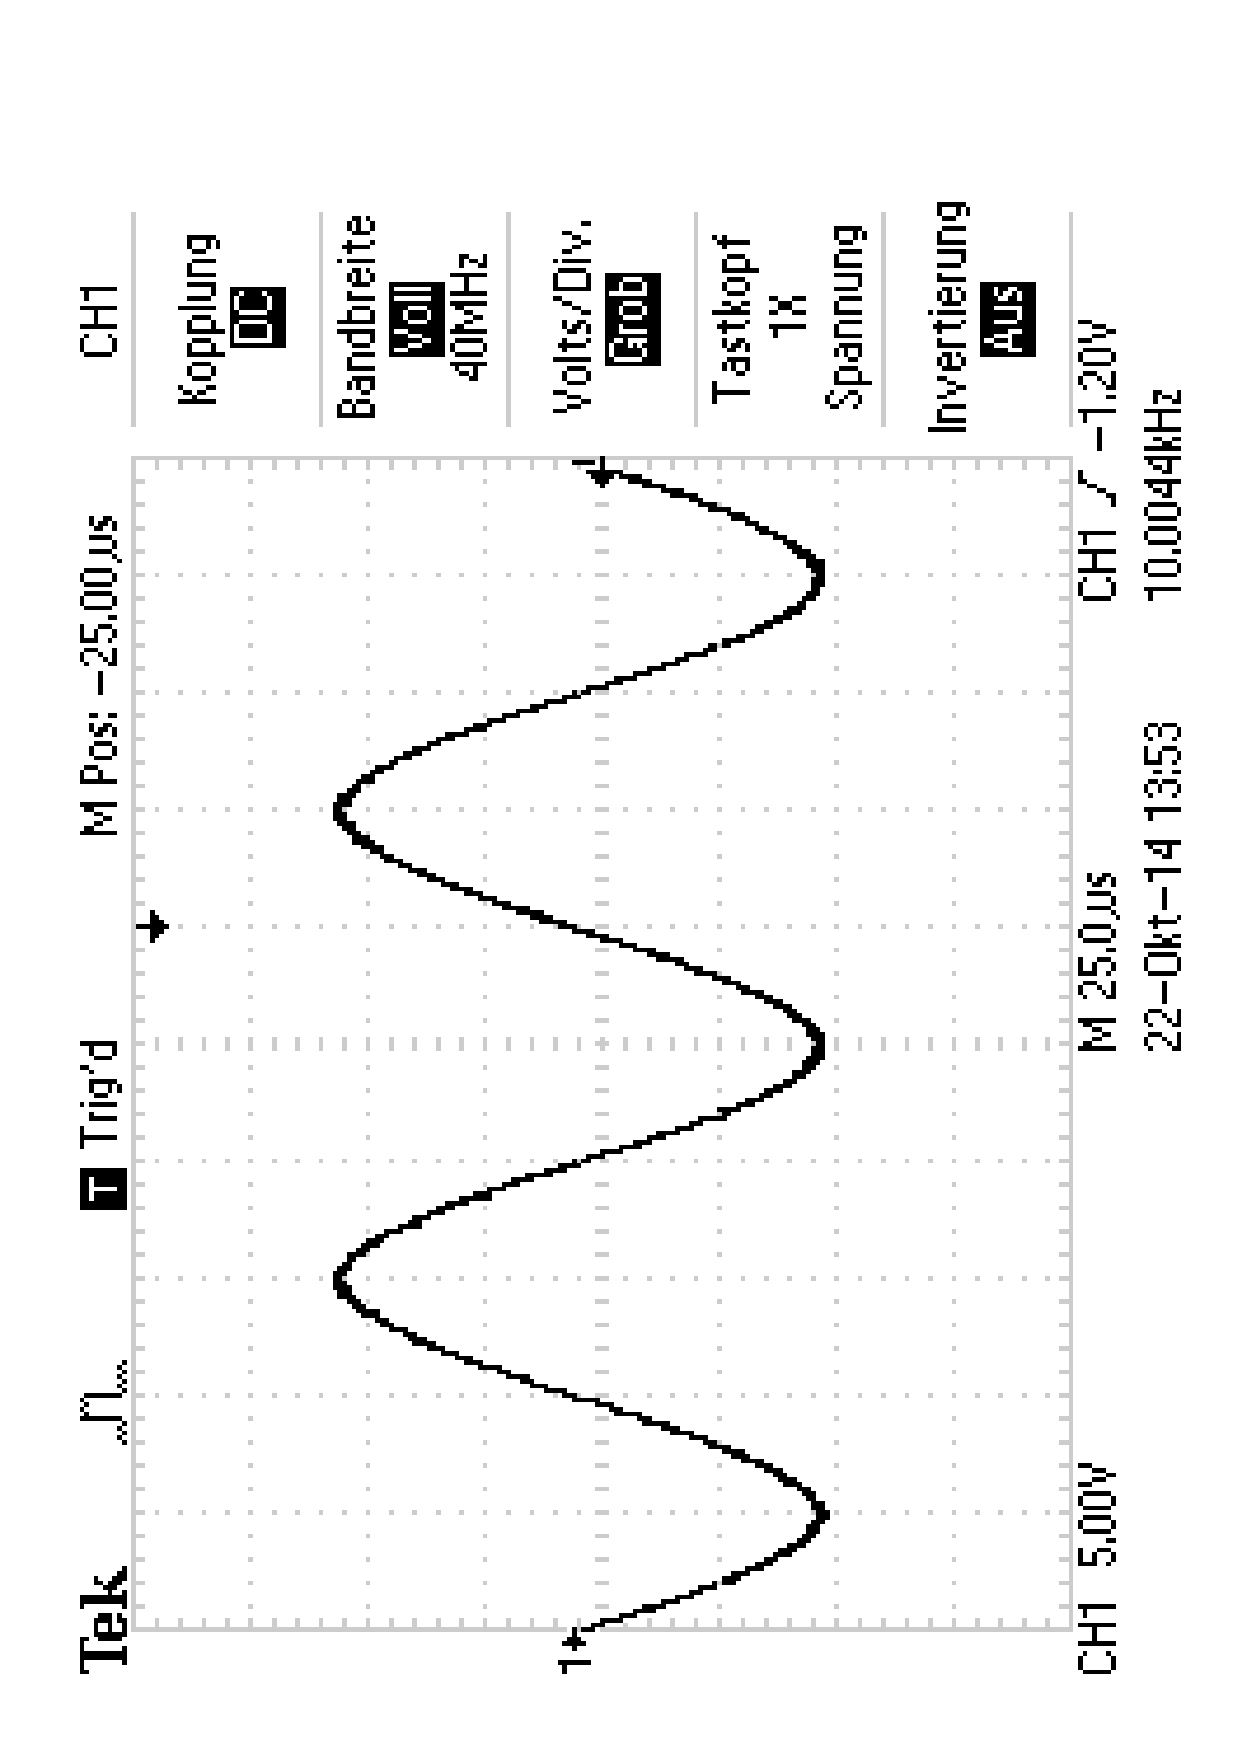
\includegraphics[trim = 0mm 50mm 0mm 50mm, clip, width=\textwidth, scale = 0.4]{TEK0011.pdf}
  \caption[Aufnahme des Signals, für delay\_10us(1)]{Aufnahme des Signals, für delay\_10us(1)} 
  \label{fig:g_6}
\end{subfigure}
\hfill
\begin{subfigure}[b]{0.28\textwidth}	
   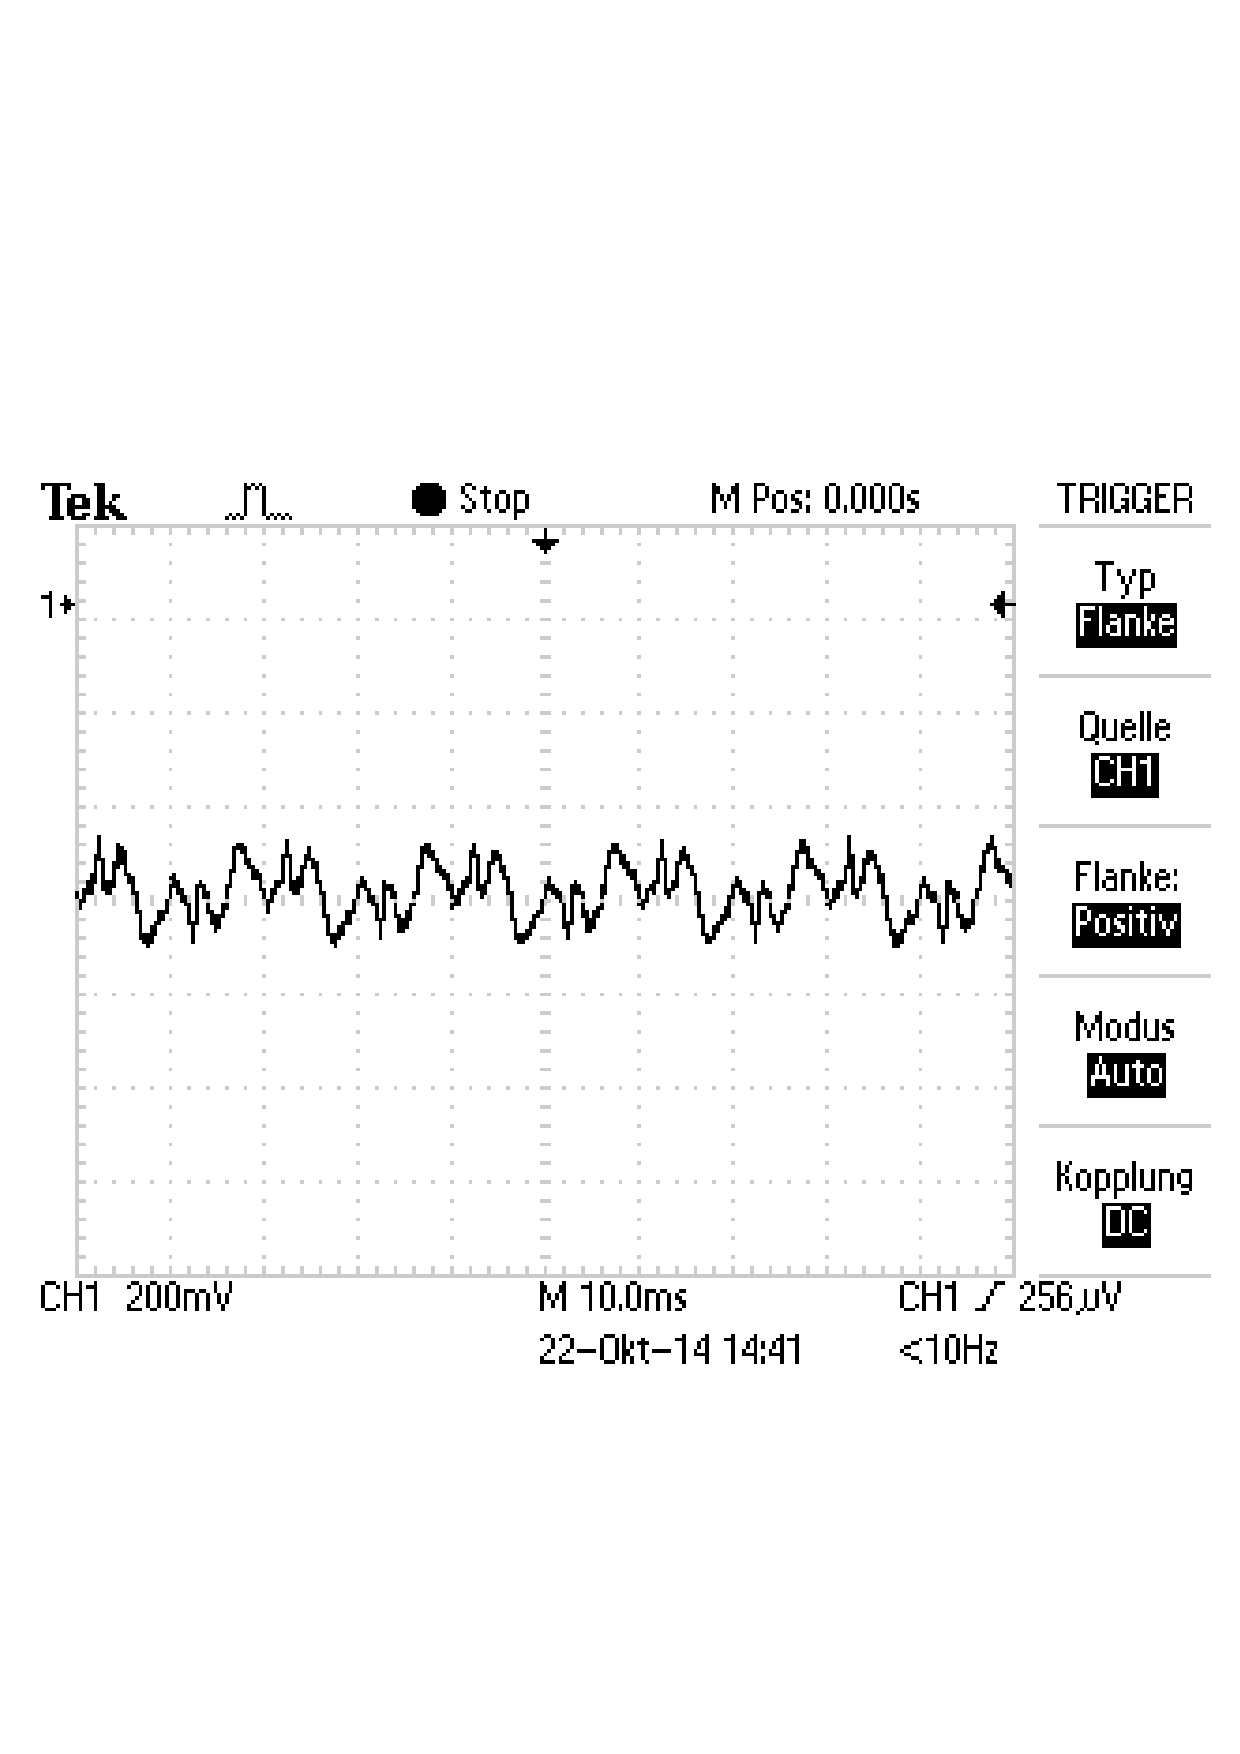
\includegraphics[trim = 0mm 50mm 0mm 50mm, clip, width=\textwidth, scale = 0.4]{TEK0012.pdf}
  \caption[Aufnahme des Signals, für delay\_ms(0)]{Aufnahme des Signals, für delay\_ms(0)} 
  \label{fig:g_7}
\end{subfigure}
\hfill
\begin{subfigure}[b]{0.28\textwidth} 	
  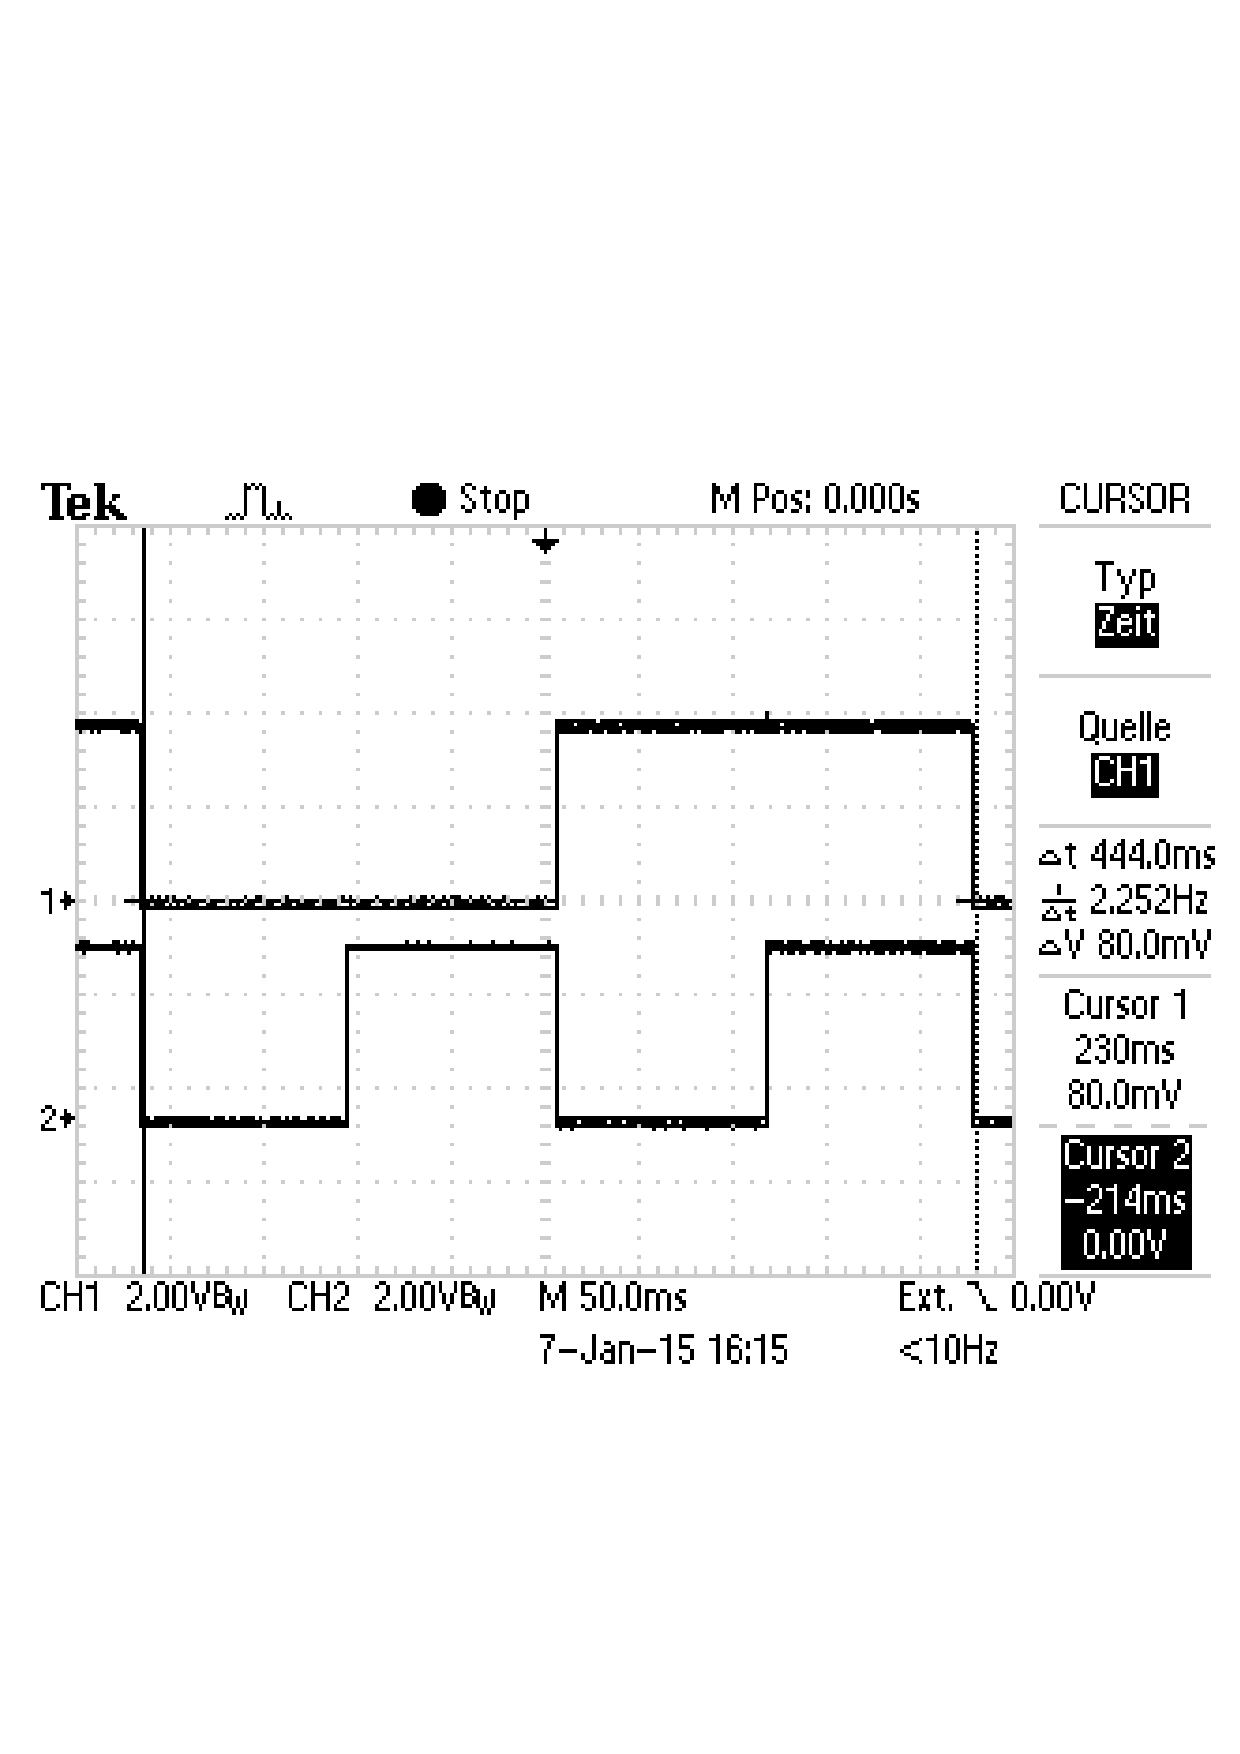
\includegraphics[trim = 0mm 50mm 0mm 50mm, clip, width=\textwidth, scale = 0.4]{TEK0013.pdf}
  \caption[Aufnahme des Signals, für delay\_ms(1)]{Aufnahme des Signals, für delay\_ms(1)} 
  \label{fig:g_8}
\end{subfigure}
\caption{Oszilloskopaufnahmen für delay\_10us(1), delay\_ms(0) und delay\_ms(1)}
\label{fig:g_main_2}
\end{figure}


\subsubsection*{Diskussion}
%(immer) die gemessenen werte und die bestimmten werte über die messfehler mit literaturwerten oder untereinander vergleichen
%in welchem fehlerintervall des messwertes liegt der literaturwert oder der vergleichswert?
%wie ist der relative anteil des fehlers am messwert und damit die qualität unserer messung?
%in einem satz erklären, wie gut unser fehler und damit unsere messung ist
%kurz erläutern, wie systematische fehler unsere messung beeinflusst haben könnten
%(wichtig) zum schluss ansprechen, in wie weit die ergebnisse mit der theoretischen vorhersage übereinstimmen
%--------------------------------------------------------------------------------------------
%falls tabellen mit den messwerten zu lang werden, kann die section mit den messwerten auch hinter der diskussion angefügt bzw. eine section mit dem anhang eingefügt werden.
%1-----------------------------------------------1


In dem Versuchsteil wurden die Methoden zur Verzögerung erfolgreich untersucht. Die Vor- und Nachteile der eizelnen Möglichkeiten zur Verzögerung konnten festgestellt werden. Mit den Delay*TCY*() Befehlen lassen sich genaue Verzögerungen realisieren, jedoch muss die Anzahl der ausgelassenen Zyklen(83,33ns) aufsummiert werden, um die Gesamtverzögerung zu erhalten. Eine bestimmte Zeit lässt sich einfacher mit den delay\_*() Befehlen umsetzen, welche bei sehr kurzen Verzögerungen eine große Ungenauigkeit haben, da der Mikrokontroller zusätzliche Zeit zur Berechnung braucht.

\section{Benutzung der Taster}
%kurz das ziel dieses versuchsteiles ansprechen, damit keine zwei überschriften direkt übereinander stehen!
%bei schwierigeren versuchen kann auch der theoretische hintergrund erläutert werden. (mit formeln, herleitungen und erklärungen)

In diesem Versuchsteil sollen Taster und deren Funktionsweise untersucht werden. Die LEDs mit den 8 Tastern sollen an- und ausgeschaltet werden, dafür wird die PollingMethode verwendet.

\subsection{Einfache Tasterabfrage}
%kurz das ziel dieses versuchsteiles ansprechen, damit keine zwei überschriften direkt übereinander stehen!
%bei schwierigeren versuchen kann auch der theoretische hintergrund erläutert werden. (mit formeln, herleitungen und erklärungen)

In diesem Versuchsteil soll die einfachste Variante eines Tasters implementiert werden. Das Programm prüft, ob der Taster gedrückt wurde, schaltet die LED ein, falls dieser gedrückt wurde.

\subsubsection*{Verwendete Geräte}
%(immer) eine skizze oder ein foto einfügen, die geräte/materialien !nummerieren! und z.b. eine legende dazu schreiben, besser wäre es das ganze in einem Fließtext gut zu beschreiben.
%falls am anfang des versuches nicht klar ist, was alles verwendet wird, wenn möglich erst am ende ein großes foto von den verwendeten materialien machen!\\

Es werden ein Netzgerät, ein PC, ein Verbindungskabel, ein Oszillsokop und das Versuchsboard verwendet.

\subsubsection*{Quellcode}

Quellcode für einen einfachen Taster.

\lstset{language=C, basicstyle=\tiny}
\begin{lstlisting}[caption = {Einfachster Version eines Schalters} \label{lst:g_5},captionpos=b]
void taster_1(){
	byte i;
	TRISB = 0b00000000;
	TRISA = 0b111111;
	
	while(1){
		i = PORTA;
		
		LATB = i;	// ueber die Variable i wird das Eingangssiganl an den Ausgang weitergegeben
	}//end of while(1)
}//end of function taster_1()
\end{lstlisting}

\subsubsection*{Versuchsdurchführung}
%erklären, !was! wir machen, !warum! wir das machen und mit welchem ziel
%(wichtig) präzize erklären, wie bei dem versuch vorgegangen und was gemacht wurde

Der Code \ref{lst:g_5} wird auf das Versuchsboard geladen, Port A wird mit den Tastern und Port B mit dem LED Port verbunden. Dann wird das Verhalten des Boards untersucht.

\subsubsection*{Auswertung}
%zuerst !alle! errechneten werte entweder in ganzen sätzen aufzählen, oder in tabellen (übersichtlicher) dargestellen, sowie auf die verwendeten formeln verweisen (die referenzierung der formel kann in der überschrift stehen)
%kurz erwähnen (vor der tabelle), warum wir das ganze ausrechnen bzw. was wir dort ausrechnen
%danach histogramme und plots erstellen, wobei wenn möglich funktionen durch die plots gelegt werden (zur not können auch splines benutzt werden, was aber angegeben werden muss)
%bei fits immer die funktion und das reduzierte chiquadrat mit angegeben, wobei auf verständlichkeit beim entziffern der zehnerpotenzen geachtet werden muss z.b. f(x)=(wert+-fehler)\cdot10^{irgendeine zahl}\cdot x + (wert+-fehler)\cdot10^{irgendeine zahl}
%bei jedem fit erklären, nach welchem zusammenhang gefittet wurde und warum!
%bei plots darauf achten, dass die achsenbeschriftung (auch die tics) die richtige größe haben und die legende im plot nicht die messwerte verdeckt
%kurz die aufgabenstellung abhandeln
%2-----------------------------------------------2

Beim Druck eines Tasters außer  Taster 4,7 und 8 leuchtete die entsprechende LED auf.

\subsection{Taster steuern Speicherfunktionen}
%kurz das ziel dieses versuchsteiles ansprechen, damit keine zwei überschriften direkt übereinander stehen!
%bei schwierigeren versuchen kann auch der theoretische hintergrund erläutert werden. (mit formeln, herleitungen und erklärungen)

In diesem Versuchsteil soll der Zustand der LED gewechselt werden, wenn der Taster gedrückt wird.

\subsubsection*{Verwendete Geräte}
%(immer) eine skizze oder ein foto einfügen, die geräte/materialien !nummerieren! und z.b. eine legende dazu schreiben, besser wäre es das ganze in einem Fließtext gut zu beschreiben.
%falls am anfang des versuches nicht klar ist, was alles verwendet wird, wenn möglich erst am ende ein großes foto von den verwendeten materialien machen!\\

Es werden ein Netzgerät, ein PC, ein Verbindungskabel, ein Oszillsokop und das Versuchsboard verwendet.

\subsubsection*{Quellcode}

Quellcode zum verwenden eines Tasters als Schalter.

\lstset{language=C, basicstyle=\tiny}
\begin{lstlisting}[caption = {Taster steuert Speicherfunktion} \label{lst:g_6},captionpos=b]
void taster_2(){
	byte i;
	TRISB = 0b00000000;
	TRISA = 0b111111;
	
	while(1){
		if(PORTA == 0b000001){	// hier wird der gesamte PORT abgefragt,
					// sodass das Druecken von zwei Tastern gleichzeitig nichts bewirkt
			if(LATB == 0b00000001)
				LATB = 0b00000000;
			else
				LATB = 0b00000001;
		}
		delay_ms(25);
	}//end of while(1)
}//end of function taster_1()

void taster_3(){
	byte i;
	TRISB = 0b00000000;
	TRISA = 0b111111;
	
	while(1){
		if(PORTAbits.RA1 == 0b1){		// nun wird nurnoch der erste Taster abgefragt,
							// unabhaengig von dem Zustand anderer Taster
			if(LATB == 0b00000001)
				LATB = 0b00000000;
			else
				LATB = 0b00000001;
		}
		delay_ms(25);
	}//end of while(1)
}//end of function taster_3()
\end{lstlisting}

\subsubsection*{Versuchsdurchführung}
%erklären, !was! wir machen, !warum! wir das machen und mit welchem ziel
%(wichtig) präzize erklären, wie bei dem versuch vorgegangen und was gemacht wurde

Der Code \ref{lst:g_6} wird auf das Versuchsboard geladen, Port A wird mit den Tastern und Port B mit dem LED Port verbunden. Dann wird das Verhalten des Boards untersucht.

\subsubsection*{Auswertung}
%zuerst !alle! errechneten werte entweder in ganzen sätzen aufzählen, oder in tabellen (übersichtlicher) dargestellen, sowie auf die verwendeten formeln verweisen (die referenzierung der formel kann in der überschrift stehen)
%kurz erwähnen (vor der tabelle), warum wir das ganze ausrechnen bzw. was wir dort ausrechnen
%danach histogramme und plots erstellen, wobei wenn möglich funktionen durch die plots gelegt werden (zur not können auch splines benutzt werden, was aber angegeben werden muss)
%bei fits immer die funktion und das reduzierte chiquadrat mit angegeben, wobei auf verständlichkeit beim entziffern der zehnerpotenzen geachtet werden muss z.b. f(x)=(wert+-fehler)\cdot10^{irgendeine zahl}\cdot x + (wert+-fehler)\cdot10^{irgendeine zahl}
%bei jedem fit erklären, nach welchem zusammenhang gefittet wurde und warum!
%bei plots darauf achten, dass die achsenbeschriftung (auch die tics) die richtige größe haben und die legende im plot nicht die messwerte verdeckt
%kurz die aufgabenstellung abhandeln
%2-----------------------------------------------2

Beim Verwenden der Funktion taster\_2() war ein schnelles Blinken der ersten LED zu sehen, falls Taster 1 gedrückt war. Wenn noch ein anderer Taster gedrückt war, während der erste Taster gedrückt wurde, blinkte die LED nicht. Beim Verwenden der Funktion taster\_3() war auch ein schnelles Blinken der LED zu sehen falls Taster 1 gedückt war. Es war auch ein Blinken zu sehen, falls ein anderer Taster gleichzeitig gedrückt wurde.

\subsection{Tasterabfrage und Verzögerungen}
%kurz das ziel dieses versuchsteiles ansprechen, damit keine zwei überschriften direkt übereinander stehen!
%bei schwierigeren versuchen kann auch der theoretische hintergrund erläutert werden. (mit formeln, herleitungen und erklärungen)

In diesem Versuchsteil soll eine Verzögerung implementiert werden, da sonst kein sauberes Umschalten möglich ist und man nur ein Flackern sehen kann.

\subsubsection*{Quellcode}

Quellcode für einen Schalter mit Verzögerung.

\lstset{language=C, basicstyle=\tiny}
\begin{lstlisting}[caption = {Tastabfrage und Verzögerung} \label{lst:g_7},captionpos=b]
void taster_4(){
	byte i;
	TRISB = 0b00000000;
	TRISA = 0b111111;
	
	while(1){
		if(PORTAbits.RA0 == 0b1){
			if(LATB == 0b00000001)
				LATB = 0b00000000;
			else
				LATB = 0b00000001;
			}
		delay_ms(500);		// um das Flackern zu verhindern wurden 500ms Delay eingebaut
	}//end of while(1)
}//end of function taster_4()
\end{lstlisting}

\subsubsection*{Versuchsdurchführung}
%erklären, !was! wir machen, !warum! wir das machen und mit welchem ziel
%(wichtig) präzize erklären, wie bei dem versuch vorgegangen und was gemacht wurde

Der Code \ref{lst:g_7} wird auf das Versuchsboard geladen, Port A wird mit den Tastern und Port B mit dem LED Port verbunden. Dann wird das Verhalten des Boards untersucht.

\subsubsection*{Auswertung}
%zuerst !alle! errechneten werte entweder in ganzen sätzen aufzählen, oder in tabellen (übersichtlicher) dargestellen, sowie auf die verwendeten formeln verweisen (die referenzierung der formel kann in der überschrift stehen)
%kurz erwähnen (vor der tabelle), warum wir das ganze ausrechnen bzw. was wir dort ausrechnen
%danach histogramme und plots erstellen, wobei wenn möglich funktionen durch die plots gelegt werden (zur not können auch splines benutzt werden, was aber angegeben werden muss)
%bei fits immer die funktion und das reduzierte chiquadrat mit angegeben, wobei auf verständlichkeit beim entziffern der zehnerpotenzen geachtet werden muss z.b. f(x)=(wert+-fehler)\cdot10^{irgendeine zahl}\cdot x + (wert+-fehler)\cdot10^{irgendeine zahl}
%bei jedem fit erklären, nach welchem zusammenhang gefittet wurde und warum!
%bei plots darauf achten, dass die achsenbeschriftung (auch die tics) die richtige größe haben und die legende im plot nicht die messwerte verdeckt
%kurz die aufgabenstellung abhandeln
%2-----------------------------------------------2

Mit dem Hinzufügen der Verzögerung konnte der Taster mit einer Frequenz von 1Hz als Schalter verwendet werden.

\subsection{Taster steuern einen Zähler}
%kurz das ziel dieses versuchsteiles ansprechen, damit keine zwei überschriften direkt übereinander stehen!
%bei schwierigeren versuchen kann auch der theoretische hintergrund erläutert werden. (mit formeln, herleitungen und erklärungen)

In diesem Versuchsteil steuert der Taster einen Zähler, welcher bei jedem Tasterndruck eine Stelle hochzählen soll.

\subsubsection*{Quellcode}

Quellcode zum steuern eines Zählers mit einem Taster.

\lstset{language=C, basicstyle=\tiny}
\begin{lstlisting}[caption = {Code zum stuern eines Zählers mit einem Schalter} \label{lst:g_9},captionpos=b]
void taster_5(){
	byte taster_alt = 0b00000000;		// taster_alt wird deklariert und definiert
	byte taster_neu = 0b00000000;		// taster_neu wird deklariert und definiert
	byte counter = 0;
	TRISB = 0b00000000;
	TRISA = 0b111111;
	
	while(1){
		taster_neu = PORTA;		// taster_neu wird der Zustand von PORTA zugewiesen
		if(taster_neu != taster_alt){	// falls taster_neu ungleich taster_alt 
						// 'falls ein Taster oder mehrere gedrueckt oder losgelassen werden'
			taster_alt = taster_neu;// setze taster_alt = taster_neu  
						//(damit auch beim Loslassen umgeschaltet wird)
			counter++;		// erhoehe den counter
			LATB = counter;		// und lasse das 8-Bit-Muster von counter am Ausgang aufleuchten
		}//end of if(taster_neu != taster_alt)
	}//end of while(1)
}//end of function taster_5()

void taster_6(){
	byte taster_alt = 0b00000000;
	byte taster_neu = 0b00000000;
	byte counter;
	byte flag = 0;			// eine Variable flag wird deklariert und definiert
	TRISB = 0b00000000;
	TRISA = 0b111111;
	
	while(1){
		taster_neu = PORTA;
		if(taster_neu != taster_alt){	// falls taster_neu ungleich taster_alt
			flag++;			// erhoehe flag um einen 
						// falls flag = 255 bzw. 11111111 ist, wird flag nun auf 0 schalten
			taster_alt = taster_neu;// und setze taster_alt = taster_neu
			if(flag%2 == 0){	// wenn dann flag modulo 2 = 0 ist
				counter++;	// erhoehe den counter
				LATB = counter;	// und gebe das Muster von counter aus
			}//end of if(flag%2 == 1)
		}//end of if(taster_neu != taster_alt)
	}//end of while(1)
}//end of function taster_6()
\end{lstlisting}

\subsubsection*{Versuchsdurchführung}
%erklären, !was! wir machen, !warum! wir das machen und mit welchem ziel
%(wichtig) präzize erklären, wie bei dem versuch vorgegangen und was gemacht wurde

Der Code \ref{lst:g_9} wird auf das Versuchsboard geladen, Port A wird mit den Tastern und Port B mit dem LED Port verbunden. Dann wird das Verhalten des Boards untersucht.

\subsubsection*{Auswertung}
%zuerst !alle! errechneten werte entweder in ganzen sätzen aufzählen, oder in tabellen (übersichtlicher) dargestellen, sowie auf die verwendeten formeln verweisen (die referenzierung der formel kann in der überschrift stehen)
%kurz erwähnen (vor der tabelle), warum wir das ganze ausrechnen bzw. was wir dort ausrechnen
%danach histogramme und plots erstellen, wobei wenn möglich funktionen durch die plots gelegt werden (zur not können auch splines benutzt werden, was aber angegeben werden muss)
%bei fits immer die funktion und das reduzierte chiquadrat mit angegeben, wobei auf verständlichkeit beim entziffern der zehnerpotenzen geachtet werden muss z.b. f(x)=(wert+-fehler)\cdot10^{irgendeine zahl}\cdot x + (wert+-fehler)\cdot10^{irgendeine zahl}
%bei jedem fit erklären, nach welchem zusammenhang gefittet wurde und warum!
%bei plots darauf achten, dass die achsenbeschriftung (auch die tics) die richtige größe haben und die legende im plot nicht die messwerte verdeckt
%kurz die aufgabenstellung abhandeln
%2-----------------------------------------------2

Bei der Implementierung von taster\_5() wurde beim Runterdrücken sowie beim Loslassen der counter um einen erhöht, dies konnte man an den LEDs sehen.
Bei der Implementierung von taster\_6() wurde nur beim Loslassen des Tasters der counter einen hochgezählt, dies war bei den LEDs zu sehen.

\subsection{Kontaktprellen der Taster -- eine Lösung}
%kurz das ziel dieses versuchsteiles ansprechen, damit keine zwei überschriften direkt übereinander stehen!
%bei schwierigeren versuchen kann auch der theoretische hintergrund erläutert werden. (mit formeln, herleitungen und erklärungen)

In diesem Versuchsteil soll der Effekt des Kontaktprellen verhindert werden. Kontaktprellen bedeutet, dass falls der Taster-Kontakt nich sauber schließt mehrfaches drücken registriert wird.

\subsubsection*{Verwendete Geräte}
%(immer) eine skizze oder ein foto einfügen, die geräte/materialien !nummerieren! und z.b. eine legende dazu schreiben, besser wäre es das ganze in einem Fließtext gut zu beschreiben.
%falls am anfang des versuches nicht klar ist, was alles verwendet wird, wenn möglich erst am ende ein großes foto von den verwendeten materialien machen!\\

Es werden ein Netzgerät, das Versuchsboard, Verbindungskabel, ein PC und ein Oszillsokop verwendet.

\subsubsection*{Quellcode}

Quellcode für die Verwendung eines Tasters als Schalter mit Unterdrückung von Kontaktprellen.

\lstset{language=C, basicstyle=\tiny}
\begin{lstlisting}[caption = {Verhindern von Kontakprellen} \label{lst:g_10},captionpos=b]
void taster_7(){
	byte taster_alt = 0b00000000;
	byte taster_neu = 0b00000000;
	byte counter = 0;
	TRISB = 0b00000000;
	TRISA = 0b111111;
	
	while(1){
		delay_ms(10);				// warte 10ms
		if(PORTA){				// falls PORTA ungleich 0
			delay_ms(10);			// warte nochmal 10ms
			while(PORTA){			// solange PORTA ungleich 0 mache nichts
			}//end of while(!PORTA)
			counter++;			// erhoehe danach counter um 1 
			LATB = counter;			// und gebe das Muster von counter am Ausgang aus
		}//end of if(taster_neu != taster_alt)
	}//end of while(1)
}//end of function taster_7()
\end{lstlisting}

\subsubsection*{Versuchsdurchführung}
%erklären, !was! wir machen, !warum! wir das machen und mit welchem ziel
%(wichtig) präzize erklären, wie bei dem versuch vorgegangen und was gemacht wurde

Der Code \ref{lst:g_10} wird auf das Versuchsboard geladen, Port A wird mit den Tastern und Port B mit dem LED Port verbunden. Dann wird das Verhalten des Boards untersucht.

\subsubsection*{Auswertung}
%zuerst !alle! errechneten werte entweder in ganzen sätzen aufzählen, oder in tabellen (übersichtlicher) dargestellen, sowie auf die verwendeten formeln verweisen (die referenzierung der formel kann in der überschrift stehen)
%kurz erwähnen (vor der tabelle), warum wir das ganze ausrechnen bzw. was wir dort ausrechnen
%danach histogramme und plots erstellen, wobei wenn möglich funktionen durch die plots gelegt werden (zur not können auch splines benutzt werden, was aber angegeben werden muss)
%bei fits immer die funktion und das reduzierte chiquadrat mit angegeben, wobei auf verständlichkeit beim entziffern der zehnerpotenzen geachtet werden muss z.b. f(x)=(wert+-fehler)\cdot10^{irgendeine zahl}\cdot x + (wert+-fehler)\cdot10^{irgendeine zahl}
%bei jedem fit erklären, nach welchem zusammenhang gefittet wurde und warum!
%bei plots darauf achten, dass die achsenbeschriftung (auch die tics) die richtige größe haben und die legende im plot nicht die messwerte verdeckt
%kurz die aufgabenstellung abhandeln
%2-----------------------------------------------2

Bei der Implementierung von Code \ref{lst:g_10} wurde beim loslassen der counter um einen erhöht, was auch an den LEDs zu sehen war.

\subsubsection*{Diskussion}
%(immer) die gemessenen werte und die bestimmten werte über die messfehler mit literaturwerten oder untereinander vergleichen
%in welchem fehlerintervall des messwertes liegt der literaturwert oder der vergleichswert?
%wie ist der relative anteil des fehlers am messwert und damit die qualität unserer messung?
%in einem satz erklären, wie gut unser fehler und damit unsere messung ist
%kurz erläutern, wie systematische fehler unsere messung beeinflusst haben könnten
%(wichtig) zum schluss ansprechen, in wie weit die ergebnisse mit der theoretischen vorhersage übereinstimmen
%--------------------------------------------------------------------------------------------
%falls tabellen mit den messwerten zu lang werden, kann die section mit den messwerten auch hinter der diskussion angefügt bzw. eine section mit dem anhang eingefügt werden.
%1-----------------------------------------------1

In diesem Versuchsteil konnten die Verwendungsmöglichkeiten, sowie verschiedene Implementierungen dieser untersucht werden. In allen Versuchsabschnitten liesen sich die gewünschten Ergebnisse erzielen.

\section{Zähler für Oszillatortakte}
%kurz das ziel dieses versuchsteiles ansprechen, damit keine zwei überschriften direkt übereinander stehen!
%bei schwierigeren versuchen kann auch der theoretische hintergrund erläutert werden. (mit formeln, herleitungen und erklärungen)

In diesem Versuchsabschnitt soll ein Zähler programmiert und implementiert werden.

\subsection{Zähler ohne Vorteiler}
%kurz das ziel dieses versuchsteiles ansprechen, damit keine zwei überschriften direkt übereinander stehen!
%bei schwierigeren versuchen kann auch der theoretische hintergrund erläutert werden. (mit formeln, herleitungen und erklärungen)

In diesem Versuchsteil wird ein Zähler ohne Vorteiler implementiert.

\subsubsection*{Verwendete Geräte}
%(immer) eine skizze oder ein foto einfügen, die geräte/materialien !nummerieren! und z.b. eine legende dazu schreiben, besser wäre es das ganze in einem Fließtext gut zu beschreiben.
%falls am anfang des versuches nicht klar ist, was alles verwendet wird, wenn möglich erst am ende ein großes foto von den verwendeten materialien machen!\\

Es werden ein Netzgerät, das Versuchsboard, Verbindungskabel, ein PC und ein Oszillsokop verwendet.

\subsubsection*{Quellcode}

Quellcode für den Zähler ohne Vorteiler.

\lstset{language=C, basicstyle=\tiny}
\begin{lstlisting}[caption = {Zähler ohne Vorteiler} \label{lst:g_11},captionpos=b]
void oszi_1(){
	byte counter = 0;
	TRISB = 0b00000000;
	TRISA = 0b111111;
	
	while(1){
		while(PORTAbits.RA0){	// solange an PORTA Spannung anliegt
			counter++;	// erhoehe den counter
			LATB = counter;	// und gebe das Muster von conter am Ausgang(LEDs) aus
		}//end of while(PORTAbits.RA0)
	}//end of function oszi_1()
}//end of while(1) und gebe das Muster von counter
\end{lstlisting}

\subsubsection*{Versuchsdurchführung}
%erklären, !was! wir machen, !warum! wir das machen und mit welchem ziel
%(wichtig) präzize erklären, wie bei dem versuch vorgegangen und was gemacht wurde

Code \ref{lst:g_11} wird auf das Versuchboard geladen. Dann wird Pin 1 von Port A mit dem Oszillator und Port B mit dem LED Port verbunden.

\subsubsection*{Auswertung}
%zuerst !alle! errechneten werte entweder in ganzen sätzen aufzählen, oder in tabellen (übersichtlicher) dargestellen, sowie auf die verwendeten formeln verweisen (die referenzierung der formel kann in der überschrift stehen)
%kurz erwähnen (vor der tabelle), warum wir das ganze ausrechnen bzw. was wir dort ausrechnen
%danach histogramme und plots erstellen, wobei wenn möglich funktionen durch die plots gelegt werden (zur not können auch splines benutzt werden, was aber angegeben werden muss)
%bei fits immer die funktion und das reduzierte chiquadrat mit angegeben, wobei auf verständlichkeit beim entziffern der zehnerpotenzen geachtet werden muss z.b. f(x)=(wert+-fehler)\cdot10^{irgendeine zahl}\cdot x + (wert+-fehler)\cdot10^{irgendeine zahl}
%bei jedem fit erklären, nach welchem zusammenhang gefittet wurde und warum!
%bei plots darauf achten, dass die achsenbeschriftung (auch die tics) die richtige größe haben und die legende im plot nicht die messwerte verdeckt
%kurz die aufgabenstellung abhandeln
%2-----------------------------------------------2

Da der Oszillator mit 60kHz getaktet ist, kann man nur ein Leuchten aller LEDs beobachten. Auf dem Oszillsokop ist der Verlauf in Abbildung \ref{fig:o_1} zu sehen. Da der Mikrocontroller eine viel höhere Taktrate als der Oszillator hat kann man während eines Taktsinals des Oszillators mehrere Zyklen des Mikrocontrollers sehen.


\begin{figure}[H] 
  \centering 	
    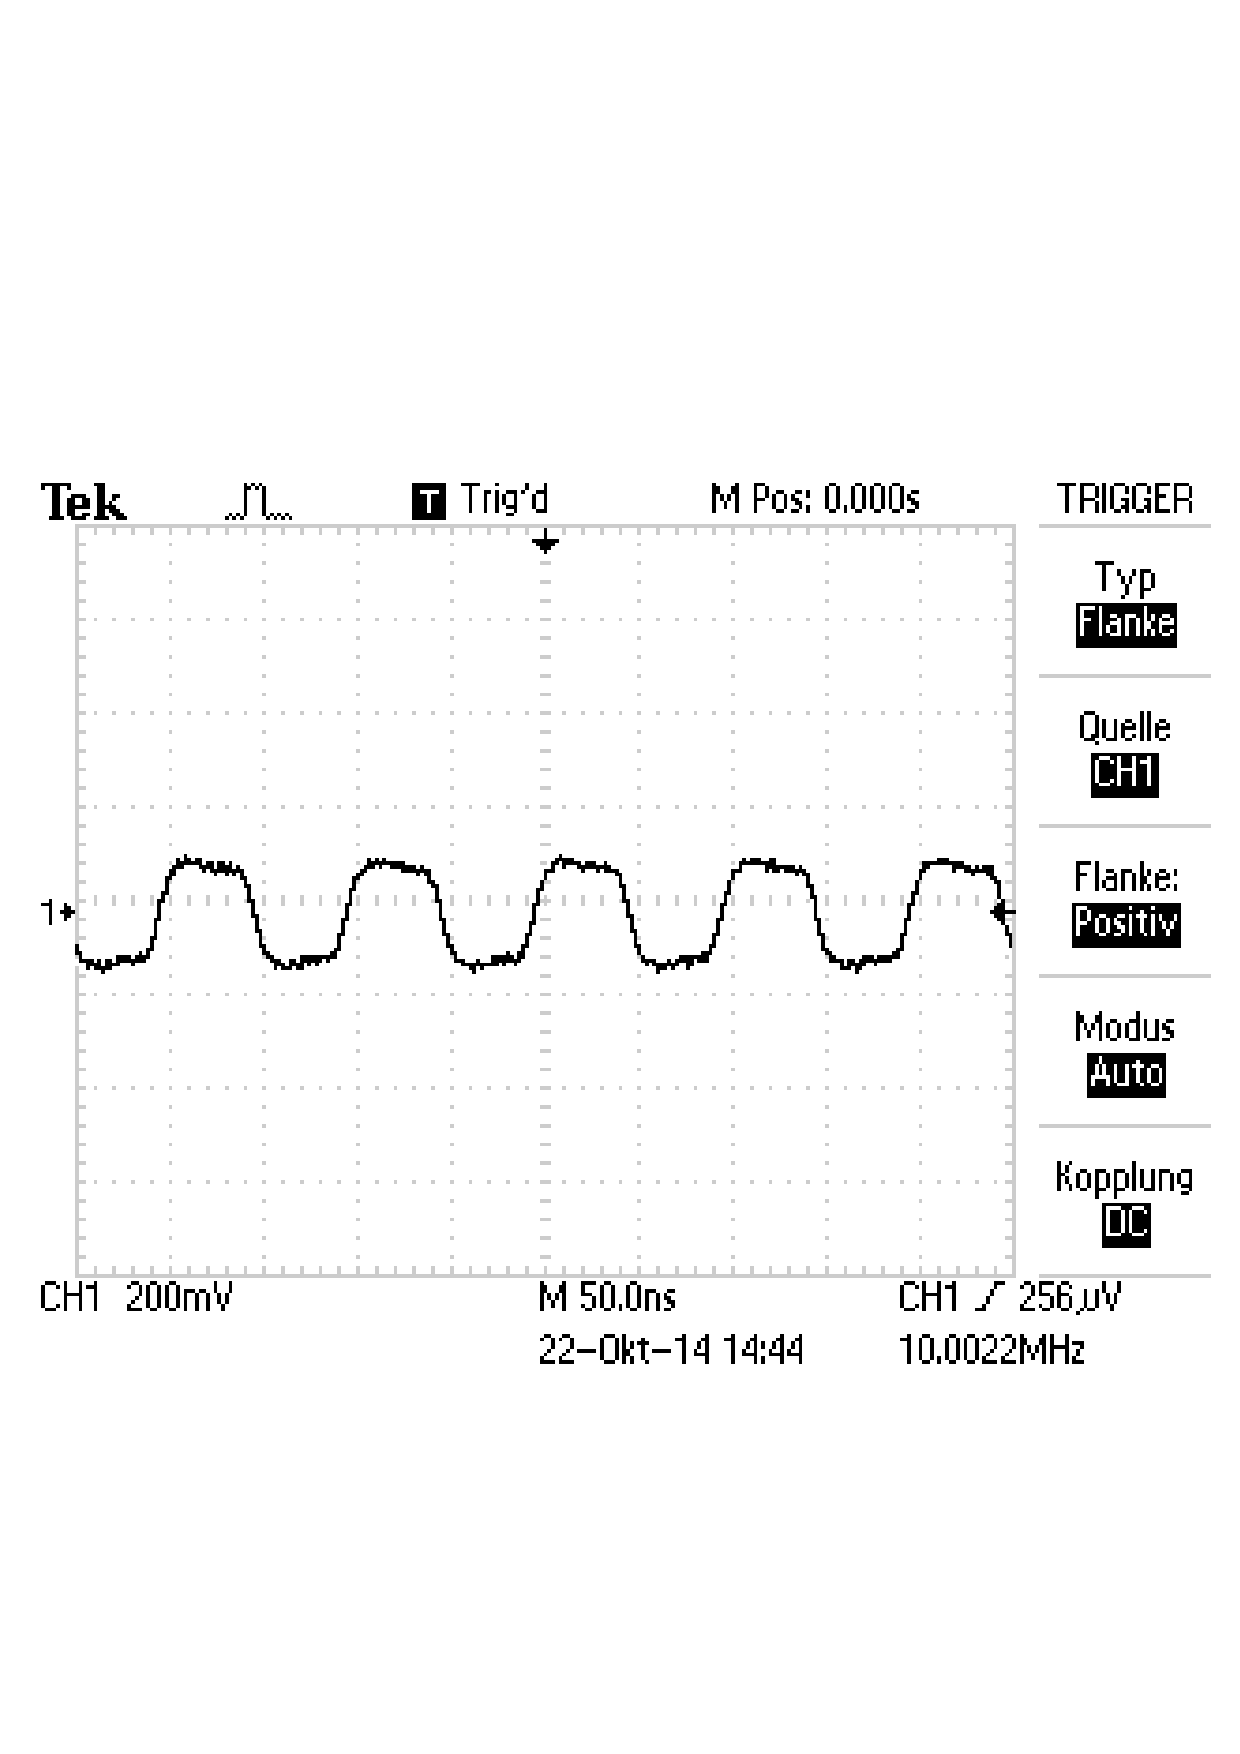
\includegraphics[trim = 0mm 50mm 0mm 50mm, clip, scale = 0.4]{TEK0014.pdf}
  	\caption[Aufnahme des Signals]{Aufnahme des Signals} 
  \label{fig:o_1}
\end{figure}

\subsection{Zähler mit Vorteiler}
%kurz das ziel dieses versuchsteiles ansprechen, damit keine zwei überschriften direkt übereinander stehen!
%bei schwierigeren versuchen kann auch der theoretische hintergrund erläutert werden. (mit formeln, herleitungen und erklärungen)

In diesem Versuchsteil soll ein Vorteiler implementiert werden, damit nicht nur ein Blinken der LEDs zu beobachten ist. Die Frequenz soll auf 5Hz geregelt werden.

\subsubsection*{Verwendete Geräte}
%(immer) eine skizze oder ein foto einfügen, die geräte/materialien !nummerieren! und z.b. eine legende dazu schreiben, besser wäre es das ganze in einem Fließtext gut zu beschreiben.
%falls am anfang des versuches nicht klar ist, was alles verwendet wird, wenn möglich erst am ende ein großes foto von den verwendeten materialien machen!\\

Es werden ein Netzgerät, das Versuchsboard, Verbindungskabel, ein PC und ein Oszillsokop verwendet.

\subsubsection*{Quellcode}

Quellcode für den Zähler mit Vorteiler.

\lstset{language=C, basicstyle=\tiny}
\begin{lstlisting}[caption = {Zähler mit Vorteiler} \label{lst:g_12},captionpos=b]
void oszi_2(){
	int i;
	byte counter = 0;
	TRISB = 0b00000000;
	TRISA = 0b111111;
	
	while(1){
		while(PORTAbits.RA0){
			for(i = 0; i < 52428; i++)
				Nop();				// warte ca. 200ms
			counter++;				// und erhoehe dann ...
			LATB = counter;
	}//end of while(1)
}//end of function oszi_2()
\end{lstlisting}

\subsubsection*{Versuchsdurchführung}
%erklären, !was! wir machen, !warum! wir das machen und mit welchem ziel
%(wichtig) präzize erklären, wie bei dem versuch vorgegangen und was gemacht wurde

Code \ref{lst:g_12} wird auf das Versuchboard geladen. Dann wird Pin 1 von Port A mit dem Oszillator und Port B mit Port LED verbunden.


\subsubsection*{Auswertung}
%zuerst !alle! errechneten werte entweder in ganzen sätzen aufzählen, oder in tabellen (übersichtlicher) dargestellen, sowie auf die verwendeten formeln verweisen (die referenzierung der formel kann in der überschrift stehen)
%kurz erwähnen (vor der tabelle), warum wir das ganze ausrechnen bzw. was wir dort ausrechnen
%danach histogramme und plots erstellen, wobei wenn möglich funktionen durch die plots gelegt werden (zur not können auch splines benutzt werden, was aber angegeben werden muss)
%bei fits immer die funktion und das reduzierte chiquadrat mit angegeben, wobei auf verständlichkeit beim entziffern der zehnerpotenzen geachtet werden muss z.b. f(x)=(wert+-fehler)\cdot10^{irgendeine zahl}\cdot x + (wert+-fehler)\cdot10^{irgendeine zahl}
%bei jedem fit erklären, nach welchem zusammenhang gefittet wurde und warum!
%bei plots darauf achten, dass die achsenbeschriftung (auch die tics) die richtige größe haben und die legende im plot nicht die messwerte verdeckt
%kurz die aufgabenstellung abhandeln
%2-----------------------------------------------2

Die LED-Anzeige zählte mit einer Frequenz von 5Hz hoch. Auf dem Oszilloskop war der Verlauf in Abbildung \ref{fig:o_2} zu sehen.

\begin{figure}[H] 
  \centering 	
    \includegraphics[trim = 0mm 50mm 0mm 50mm, clip, scale = 0.4]{TEK0015.pdf}
  	\caption[Aufnahme des Signals]{Aufnahme des Signals} 
  \label{fig:o_2}
\end{figure}

\subsubsection*{Diskussion}
%(immer) die gemessenen werte und die bestimmten werte über die messfehler mit literaturwerten oder untereinander vergleichen
%in welchem fehlerintervall des messwertes liegt der literaturwert oder der vergleichswert?
%wie ist der relative anteil des fehlers am messwert und damit die qualität unserer messung?
%in einem satz erklären, wie gut unser fehler und damit unsere messung ist
%kurz erläutern, wie systematische fehler unsere messung beeinflusst haben könnten
%(wichtig) zum schluss ansprechen, in wie weit die ergebnisse mit der theoretischen vorhersage übereinstimmen
%--------------------------------------------------------------------------------------------
%falls tabellen mit den messwerten zu lang werden, kann die section mit den messwerten auch hinter der diskussion angefügt bzw. eine section mit dem anhang eingefügt werden.
%1-----------------------------------------------1

In diesem Versuchsabschnitt konnte die Verwendungsmöglichkeit eines Oszillators beobachtet werden.

\section{Verwendung des Analog-Digital-Konverters (ADC)}
%kurz das ziel dieses versuchsteiles ansprechen, damit keine zwei überschriften direkt übereinander stehen!
%bei schwierigeren versuchen kann auch der theoretische hintergrund erläutert werden. (mit formeln, herleitungen und erklärungen)

Der Mikrocontroller besitzt einen ADC, mit dem Spannungen von 0 bis 5V gemessen werden können. In diesem Versuchsabschnitt soll damit ein Voltmeter gebaut werden.

\subsection{Anzeige des ADC-Wertes auf 8 LEDs}
%kurz das ziel dieses versuchsteiles ansprechen, damit keine zwei überschriften direkt übereinander stehen!
%bei schwierigeren versuchen kann auch der theoretische hintergrund erläutert werden. (mit formeln, herleitungen und erklärungen)

In diesem Versuchsteil soll die einfachste Version eines Voltmeters implementiert werden. Zur Ausgabe werden die 8 LEDs verwendet.

\subsubsection*{Verwendete Geräte}
%(immer) eine skizze oder ein foto einfügen, die geräte/materialien !nummerieren! und z.b. eine legende dazu schreiben, besser wäre es das ganze in einem Fließtext gut zu beschreiben.
%falls am anfang des versuches nicht klar ist, was alles verwendet wird, wenn möglich erst am ende ein großes foto von den verwendeten materialien machen!\\

Es werden das Versuchsboard, Verbindungskabel, ein PC und ein Netzgerät verwendet.


\subsubsection*{Quellcode}

Quellcode für den ADC mit LEDs.

\lstset{language=C, basicstyle=\tiny}
\begin{lstlisting}[caption = {adc mit LEDs} \label{lst:g_13},captionpos=b]
void adc_1(){
	TRISB = 0b00000000;
	TRISAbits.TRISA0 = 0b1;
	
	setup_adc_ports(AN0_TO_AN1);
	
	setup_adc(ADC_CLOCK_DIV_32);
	
	set_adc_channel(0);
	
	read_adc(ADC_START_ONLY);
	
	while(1){
		delay_ms(10);			// warte 10ms
		LATB = (read_adc(ADC_READ)>>2);	// dann uebersetze den Spannungswert in ein 8 Bit Muster und zeige es an
	}//end of while(1)
}//end of function adc_1()
\end{lstlisting}

\subsubsection*{Versuchsdurchführung}
%erklären, !was! wir machen, !warum! wir das machen und mit welchem ziel
%(wichtig) präzize erklären, wie bei dem versuch vorgegangen und was gemacht wurde

Der Code \ref{lst:g_13} wird auf den Mikrocontroller geladen und eine Spannung an AN0 angelegt. Die externe Spannung wird auf 0 und 5 V eingestellt und dann mit dem Board gemessen. Dann soll noch die Spannung ermittelt werden, bei dem das  Board den maximalen und den halben maximalen Wert anzeigt.(Abhängig von den LEDs.)


\subsubsection*{Auswertung}
%zuerst !alle! errechneten werte entweder in ganzen sätzen aufzählen, oder in tabellen (übersichtlicher) dargestellen, sowie auf die verwendeten formeln verweisen (die referenzierung der formel kann in der überschrift stehen)
%kurz erwähnen (vor der tabelle), warum wir das ganze ausrechnen bzw. was wir dort ausrechnen
%danach histogramme und plots erstellen, wobei wenn möglich funktionen durch die plots gelegt werden (zur not können auch splines benutzt werden, was aber angegeben werden muss)
%bei fits immer die funktion und das reduzierte chiquadrat mit angegeben, wobei auf verständlichkeit beim entziffern der zehnerpotenzen geachtet werden muss z.b. f(x)=(wert+-fehler)\cdot10^{irgendeine zahl}\cdot x + (wert+-fehler)\cdot10^{irgendeine zahl}
%bei jedem fit erklären, nach welchem zusammenhang gefittet wurde und warum!
%bei plots darauf achten, dass die achsenbeschriftung (auch die tics) die richtige größe haben und die legende im plot nicht die messwerte verdeckt
%kurz die aufgabenstellung abhandeln
%2-----------------------------------------------2

Bei 0V waren alle LEDs aus, entspricht also einer dezimalen 0. Bei 5V waren alle LEDs an, was einem dezimalen Wert von 255 entspricht. Dies war gleichzeitig der Maximalwert. Der halbe Maximalwert wurde bei 2,4V angezeigt.

\subsection{Anzeige des ADC-Wertes auf der Siebensegmentanzeige}
%kurz das ziel dieses versuchsteiles ansprechen, damit keine zwei überschriften direkt übereinander stehen!
%bei schwierigeren versuchen kann auch der theoretische hintergrund erläutert werden. (mit formeln, herleitungen und erklärungen)

In diesem Versuchsteil soll die gemessene Spannung mit einer Siebensegmentanzeige ausgegeben werden.

\subsubsection*{Verwendete Geräte}
%(immer) eine skizze oder ein foto einfügen, die geräte/materialien !nummerieren! und z.b. eine legende dazu schreiben, besser wäre es das ganze in einem Fließtext gut zu beschreiben.
%falls am anfang des versuches nicht klar ist, was alles verwendet wird, wenn möglich erst am ende ein großes foto von den verwendeten materialien machen!\\

Es werden das Versuchsboard, Verbindungskabel, ein PC und ein Netzgerät verwendet.

\subsubsection*{Quellcode}

Quellcode für die Ausgabe des ADC mit einer Siebensegmanetanzeige.

\lstset{language=C, basicstyle=\tiny}
\begin{lstlisting}[caption = {adc mit Siebensegmentanzeige} \label{lst:g_14},captionpos=b]
void adc_2(){
	char value;
	byte valH;
	byte valL;

	TRISD = 0b00000000;
	TRISC = 0b00000000;
	TRISB = 0b00000000;
	TRISAbits.TRISA0 = 1;

	setup_adc_ports(AN0_TO_AN1);
	
	setup_adc(ADC_CLOCK_DIV_32);
	
	set_adc_channel(0);
	
	read_adc(ADC_START_ONLY);
	
	while(1){
		delay_ms(10);
		
		value = read_adc(ADC_READ)>>2;
		
		valH = value>>4;
		valL = (value & 0b00001111)>>4;
		
		LATD = dec_7seg[valH];
		LATC = dec_7seg[valL];
		
	}//end of while(1)
}//end of function adc_2()
\end{lstlisting}

\subsubsection*{Versuchsdurchführung}
%erklären, !was! wir machen, !warum! wir das machen und mit welchem ziel
%(wichtig) präzize erklären, wie bei dem versuch vorgegangen und was gemacht wurde

Der Code \ref{lst:g_14} wird auf den Mikrocontroller geladen und eine Spannung an AN0 angelegt. Die externe Spannung wird auf 0 und 5 V eingestellt und dann mit dem Board gemessen. Dann soll noch die Spannung ermittelt werden, bei dem das  Board den maximalen und den mittleren Wert anzeigt.

\subsubsection*{Auswertung}
%zuerst !alle! errechneten werte entweder in ganzen sätzen aufzählen, oder in tabellen (übersichtlicher) dargestellen, sowie auf die verwendeten formeln verweisen (die referenzierung der formel kann in der überschrift stehen)
%kurz erwähnen (vor der tabelle), warum wir das ganze ausrechnen bzw. was wir dort ausrechnen
%danach histogramme und plots erstellen, wobei wenn möglich funktionen durch die plots gelegt werden (zur not können auch splines benutzt werden, was aber angegeben werden muss)
%bei fits immer die funktion und das reduzierte chiquadrat mit angegeben, wobei auf verständlichkeit beim entziffern der zehnerpotenzen geachtet werden muss z.b. f(x)=(wert+-fehler)\cdot10^{irgendeine zahl}\cdot x + (wert+-fehler)\cdot10^{irgendeine zahl}
%bei jedem fit erklären, nach welchem zusammenhang gefittet wurde und warum!
%bei plots darauf achten, dass die achsenbeschriftung (auch die tics) die richtige größe haben und die legende im plot nicht die messwerte verdeckt
%kurz die aufgabenstellung abhandeln
%2-----------------------------------------------2

Bei 0V wurde der Wert 0 auf der Siebensegmentanzeige angezeigt. Der Maximale Wert F wurde zum ersten mal bei 4,6V gemessen, bei 5V wurde auch F angezeigt. F entspricht der dezimalzahl 15. Der halbe maximale Wert wurde bei 2,3V angezeigt und entspricht einer Dezimalzahl von 7;

\subsection{Anzeige von zwei ADC-Kanälen auf der Siebensegmentanzeige}
%kurz das ziel dieses versuchsteiles ansprechen, damit keine zwei überschriften direkt übereinander stehen!
%bei schwierigeren versuchen kann auch der theoretische hintergrund erläutert werden. (mit formeln, herleitungen und erklärungen)

In diesem Versuchsteil soll noch die Funktion implementiert werden, mit der per Tasterdruck zwischen den Kanälen AN0 und AN1 umschalten kann.

\subsubsection*{Verwendete Geräte}
%(immer) eine skizze oder ein foto einfügen, die geräte/materialien !nummerieren! und z.b. eine legende dazu schreiben, besser wäre es das ganze in einem Fließtext gut zu beschreiben.
%falls am anfang des versuches nicht klar ist, was alles verwendet wird, wenn möglich erst am ende ein großes foto von den verwendeten materialien machen!\\

Es werden das Versuchsboard, Verbindungskabel, ein PC und ein Netzgerät verwendet.

\subsubsection*{Quellcode}

Quellcode für adc Messung mit Umschaltfunktion.

\lstset{language=C, basicstyle=\tiny}
\begin{lstlisting}[caption = {acd mit Umschaltfunktion} \label{lst:g_15},captionpos=b]
void adc_3(){
	byte flag = 0;

	TRISC = 0b11111111;
	TRISB = 0b00000000;
	TRISAbits.TRISA0 = 1;
	TRISAbits.TRISA1 = 1;
	
	
	//setting up the adc
	setup_adc_ports(AN0_TO_AN1);
	setup_adc(ADC_CLOCK_DIV_32);
	set_adc_channel(0);
	read_adc(ADC_START_ONLY);
	
	//starting the main routine
	while(1){
		if(PORTCbits.RC0 == 0b1){
			if(flag == 0)
				flag = 1;
			else
				flag = 0;
			}//end of if(PORTCbits.RC0 == 0b1)
		if(flag == 0){
			set_adc_channel(0);
			read_adc(ADC_START_ONLY);
		} else {
			set_adc_channel(1);
			read_adc(ADC_START_ONLY);			
		}
		
		delay_ms(100);
		
		LATB = read_adc(ADC_READ)<<2;
		
		delay_ms(1000);
				
	}//end of while(1)
}//end of function adc_3()
\end{lstlisting}

\subsubsection*{Versuchsdurchführung}
%erklären, !was! wir machen, !warum! wir das machen und mit welchem ziel
%(wichtig) präzize erklären, wie bei dem versuch vorgegangen und was gemacht wurde

Der Code \ref{lst:g_15} wird auf den Mikrocontroller geladen und überprüft, ob das Programm wie erwartet funktioniert.

\subsubsection*{Auswertung}
%zuerst !alle! errechneten werte entweder in ganzen sätzen aufzählen, oder in tabellen (übersichtlicher) dargestellen, sowie auf die verwendeten formeln verweisen (die referenzierung der formel kann in der überschrift stehen)
%kurz erwähnen (vor der tabelle), warum wir das ganze ausrechnen bzw. was wir dort ausrechnen
%danach histogramme und plots erstellen, wobei wenn möglich funktionen durch die plots gelegt werden (zur not können auch splines benutzt werden, was aber angegeben werden muss)
%bei fits immer die funktion und das reduzierte chiquadrat mit angegeben, wobei auf verständlichkeit beim entziffern der zehnerpotenzen geachtet werden muss z.b. f(x)=(wert+-fehler)\cdot10^{irgendeine zahl}\cdot x + (wert+-fehler)\cdot10^{irgendeine zahl}
%bei jedem fit erklären, nach welchem zusammenhang gefittet wurde und warum!
%bei plots darauf achten, dass die achsenbeschriftung (auch die tics) die richtige größe haben und die legende im plot nicht die messwerte verdeckt
%kurz die aufgabenstellung abhandeln
%2-----------------------------------------------2

Beim drücken des Schalters wurde wie erwartet der Kanal an dem die Spannung gemessen wurde gewechselt. Aufgrund der langen Verzögerung musste immer ein Moment gewartet werden, bis der Kanal wieder gewechselt werden konnte.

\subsection{Anzeige des ADC-Wertes auf einer Balkenanzeige}
%kurz das ziel dieses versuchsteiles ansprechen, damit keine zwei überschriften direkt übereinander stehen!
%bei schwierigeren versuchen kann auch der theoretische hintergrund erläutert werden. (mit formeln, herleitungen und erklärungen)

In diesem Versuchsteil soll die gemessene Spannung mit einer Balkenanzeige angezeigt werden.

\subsubsection*{Verwendete Geräte}
%(immer) eine skizze oder ein foto einfügen, die geräte/materialien !nummerieren! und z.b. eine legende dazu schreiben, besser wäre es das ganze in einem Fließtext gut zu beschreiben.
%falls am anfang des versuches nicht klar ist, was alles verwendet wird, wenn möglich erst am ende ein großes foto von den verwendeten materialien machen!\\

Es werden das Versuchsboard, Verbindungskabel, ein PC und ein Netzgerät verwendet.

\subsubsection*{Quellcode}

Quellcode für adc mit Balkenanzeige.

\lstset{language=C, basicstyle=\tiny}
\begin{lstlisting}[caption = {adc mit Balkenanzeige} \label{lst:g_16},captionpos=b]
void adc_4(){
	byte val;
	
	TRISB = 0b00000000;
	TRISAbits.TRISA0 = 0b1;
	
	setup_adc_ports(AN0_TO_AN1);
	setup_adc(ADC_CLOCK_DIV_32);
	set_adc_channel(0);
	read_adc(ADC_START_ONLY);
	
	while(1){
		delay_ms(10);
		val = (read_adc(ADC_READ)>>7);	//Es werden nur die letzen drei bits verwendet,
						//da sich darus acht moegliche Zustaende ergeben
						//Die Zustaende muessen alle einzeln ausgewertet werden
		if(val == 0b00000000)
			LATB = 0b00000000;		
		if(val == 0b00000001)
			LATB = 0b00000001;
		if(val == 0b00000010)
			LATB = 0b00000011;
		if(val == 0b00000011)
			LATB = 0b00000111;		
		if(val == 0b00000111)
			LATB = 0b00001111;
		if(val == 0b00000100)
			LATB = 0b00011111;
		if(val == 0b00000101)
			LATB = 0b00111111;
		if(val == 0b00000110)
			LATB = 0b01111111;		
		if(val == 0b00000111)
			LATB = 0b11111111;					
	}//end of while(1)
}//end of function adc_4()
\end{lstlisting}

\subsubsection*{Versuchsdurchführung}
%erklären, !was! wir machen, !warum! wir das machen und mit welchem ziel
%(wichtig) präzize erklären, wie bei dem versuch vorgegangen und was gemacht wurde

Der Code \ref{lst:g_16} wird auf den Mikrocontroller geladen und das Verhalten untersucht.

\subsubsection*{Auswertung}
%zuerst !alle! errechneten werte entweder in ganzen sätzen aufzählen, oder in tabellen (übersichtlicher) dargestellen, sowie auf die verwendeten formeln verweisen (die referenzierung der formel kann in der überschrift stehen)
%kurz erwähnen (vor der tabelle), warum wir das ganze ausrechnen bzw. was wir dort ausrechnen
%danach histogramme und plots erstellen, wobei wenn möglich funktionen durch die plots gelegt werden (zur not können auch splines benutzt werden, was aber angegeben werden muss)
%bei fits immer die funktion und das reduzierte chiquadrat mit angegeben, wobei auf verständlichkeit beim entziffern der zehnerpotenzen geachtet werden muss z.b. f(x)=(wert+-fehler)\cdot10^{irgendeine zahl}\cdot x + (wert+-fehler)\cdot10^{irgendeine zahl}
%bei jedem fit erklären, nach welchem zusammenhang gefittet wurde und warum!
%bei plots darauf achten, dass die achsenbeschriftung (auch die tics) die richtige größe haben und die legende im plot nicht die messwerte verdeckt
%kurz die aufgabenstellung abhandeln
%2-----------------------------------------------2

Da nicht genug Zeit zur verfügung stand, konnte der Code nicht am Board getestet werden. Der Code sollte lauffähig sein und aus der LED-Anzeige eine Balkenanzeige machen.

\section{Fazit}
%im fazit nochmal alles zusammenfassen und den verlauf der messung abschätzen
%gravierende sytematische probleme bei den messungen nochmal betonen und die wertigkeit unserer ergebnisse einordnen


\end{document}

